% ******************************* PhD Thesis Template **************************
% Please have a look at the README.md file for info on how to use the template

\documentclass[a4paper,12pt,custombib,print,draft,index]{PhDThesisPSnPDF}

% ******************************************************************************
% ******************************* Class Options ********************************
% *********************** See README for more details **************************
% ******************************************************************************

% `a4paper'(The University of Cambridge PhD thesis guidelines recommends a page
% size a4 - default option) or `a5paper': A5 Paper size is also allowed as per
% the Cambridge University Engineering Deparment guidelines for PhD thesis
%
% `11pt' or `12pt'(default): Font Size 10pt is NOT recommended by the University
% guidelines
%
% `oneside' or `twoside'(default): Printing double side (twoside) or single
% side.
%
% `print': Use `print' for print version with appropriate margins and page
% layout. Leaving the options field blank will activate Online version.
%
% `index': For index at the end of the thesis
%
% `draftclassic': For draft mode without loading any images (same as draft in book)
%
% `draft': Special draft mode with line numbers, images, and water mark with
% timestamp and custom text. Position of the text can also be modified.
%
% `abstract': To generate only the title page and abstract page with
% dissertation title and name, to submit to the Student Registry
%
% `chapter`: This option enables only the specified chapter and its references
%  Useful for review and corrections.
%
% ************************* Custom Page Margins ********************************
%
% `custommargin`: Use `custommargin' in options to activate custom page margins,
% which can be defined in the preamble.tex. Custom margin will override
% print/online margin setup.
%
% *********************** Choosing the Fonts in Class Options ******************
%
% `times' : Times font with math support. (The Cambridge University guidelines
% recommend using times)
%
% `fourier': Utopia Font with Fourier Math font (Font has to be installed)
%            It's a free font.
%
% `customfont': Use `customfont' option in the document class and load the
% package in the preamble.tex
%
% default or leave empty: `Latin Modern' font will be loaded.
%
% ********************** Choosing the Bibliography style ***********************
%
% `authoryear': For author-year citation eg., Krishna (2013)
%
% `numbered': (Default Option) For numbered and sorted citation e.g., [1,5,2]
%
% `custombib': Define your own bibliography style in the `preamble.tex' file.
%              `\RequirePackage[square, sort, numbers, authoryear]{natbib}'.
%              This can be also used to load biblatex instead of natbib
%              (See Preamble)
%
% **************************** Choosing the Page Style *************************
%
% `default (leave empty)': For Page Numbers in Header (Left Even, Right Odd) and
% Chapter Name in Header (Right Even) and Section Name (Left Odd). Blank Footer.
%
% `PageStyleI': Chapter Name next & Page Number on Even Side (Left Even).
% Section Name & Page Number in Header on Odd Side (Right Odd). Footer is empty.
%
% `PageStyleII': Chapter Name on Even Side (Left Even) in Header. Section Number
% and Section Name in Header on Odd Side (Right Odd). Page numbering in footer

% Uncomment to change page style
%\pagestyle{PageStyleII}

% ********************************** Preamble **********************************
% Preamble: Contains packages and user-defined commands and settings
% ******************************************************************************
% ****************************** Custom Margin *********************************

% Add `custommargin' in the document class options to use this section
% Set {innerside margin / outerside margin / topmargin / bottom margin}  and
% other page dimensions
\ifsetCustomMargin
  \RequirePackage[left=37mm,right=30mm,top=35mm,bottom=30mm]{geometry}
  \setFancyHdr % To apply fancy header after geometry package is loaded
\fi

% Add spaces between paragraphs
%\setlength{\parskip}{0.5em}
% Ragged bottom avoids extra whitespaces between paragraphs
\raggedbottom
% To remove the excess top spacing for enumeration, list and description
%\usepackage{enumitem}
%\setlist[enumerate,itemize,description]{topsep=0em}

% *****************************************************************************
% ******************* Fonts (like different typewriter fonts etc.)*************

% Add `customfont' in the document class option to use this section

\ifsetCustomFont
  % Set your custom font here and use `customfont' in options. Leave empty to
  % load computer modern font (default LaTeX font).
  %\RequirePackage{helvet}

  % For use with XeLaTeX
  %  \setmainfont[
  %    Path              = ./libertine/opentype/,
  %    Extension         = .otf,
  %    UprightFont = LinLibertine_R,
  %    BoldFont = LinLibertine_RZ, % Linux Libertine O Regular Semibold
  %    ItalicFont = LinLibertine_RI,
  %    BoldItalicFont = LinLibertine_RZI, % Linux Libertine O Regular Semibold Italic
  %  ]
  %  {libertine}
  %  % load font from system font
  %  \newfontfamily\libertinesystemfont{Linux Libertine O}
\fi

% *****************************************************************************
% **************************** Custom Packages ********************************

% ************************* Algorithms and Pseudocode **************************

%\usepackage{algpseudocode}


% ********************Captions and Hyperreferencing / URL **********************

% Captions: This makes captions of figures use a boldfaced small font.
%\RequirePackage[small,bf]{caption}

\RequirePackage[labelsep=space,tableposition=top]{caption}
\renewcommand{\figurename}{Fig.} %to support older versions of captions.sty

\usepackage{hyperref}

% *************************** Graphics and figures *****************************

%\usepackage{rotating}
%\usepackage{wrapfig}

% Uncomment the following two lines to force Latex to place the figure.
% Use [H] when including graphics. Note 'H' instead of 'h'
%\usepackage{float}
%\restylefloat{figure}

% Subcaption package is also available in the sty folder you can use that by
% uncommenting the following line
% This is for people stuck with older versions of texlive
%\usepackage{sty/caption/subcaption}
\usepackage{subcaption}

% ********************************** Tables ************************************
\usepackage{booktabs} % For professional looking tables
\usepackage{multirow}

%\usepackage{multicol}
%\usepackage{longtable}
%\usepackage{tabularx}


% *********************************** SI Units *********************************
\usepackage{siunitx} % use this package module for SI units
\sisetup{separate-uncertainty = true, range-phrase = --, range-units = single, group-separator = {,}}
\DeclareSIUnit\npe{\text{npe}}

% ******************************* Line Spacing *********************************

% Choose linespacing as appropriate. Default is one-half line spacing as per the
% University guidelines

\doublespacing
% \onehalfspacing
% \singlespacing


% ************************ Formatting / Footnote *******************************

% Don't break enumeration (etc.) across pages in an ugly manner (default 10000)
%\clubpenalty=500
%\widowpenalty=500

%\usepackage[perpage]{footmisc} %Range of footnote options


% *****************************************************************************
% *************************** Bibliography  and References ********************

%\usepackage{cleveref} %Referencing without need to explicitly state fig /table

% Add `custombib' in the document class option to use this section
\ifuseCustomBib
   \RequirePackage[square, sort, numbers]{natbib} % CustomBib [square, sort, numbers, authoryear]

% If you would like to use biblatex for your reference management, as opposed to the default `natbibpackage` pass the option `custombib` in the document class. Comment out the previous line to make sure you don't load the natbib package. Uncomment the following lines and specify the location of references.bib file

% \RequirePackage[
%   backend=biber,
%   % style=numeric-comp,
%   style=phys,
%   % citestyle=numeric,
%   % sorting=nty,
%   % natbib=true
%   maxnames=4,
%   bibencoding=utf8
%   ]{biblatex}
% \addbibresource{References/references.bib} %Location of references.bib only for biblatex, Do not omit the .bib extension from the filename.

\fi

% changes the default name `Bibliography` -> `References'
\renewcommand{\bibname}{References}


% ******************************************************************************
% ************************* User Defined Commands ******************************
% ******************************************************************************

% *********** To change the name of Table of Contents / LOF and LOT ************

%\renewcommand{\contentsname}{My Table of Contents}
%\renewcommand{\listfigurename}{My List of Figures}
%\renewcommand{\listtablename}{My List of Tables}


% ********************** TOC depth and numbering depth *************************

\setcounter{secnumdepth}{2}
\setcounter{tocdepth}{2}


% ******************************* Nomenclature *********************************

% To change the name of the Nomenclature section, uncomment the following line

%\renewcommand{\nomname}{Symbols}


% ********************************* Appendix ***********************************

% The default value of both \appendixtocname and \appendixpagename is `Appendices'. These names can all be changed via:

%\renewcommand{\appendixtocname}{List of appendices}
%\renewcommand{\appendixname}{Appndx}

% *********************** Configure Draft Mode **********************************

% Uncomment to disable figures in `draft'
%\setkeys{Gin}{draft=true}  % set draft to false to enable figures in `draft'

% These options are active only during the draft mode
% Default text is "Draft"
%\SetDraftText{DRAFT}

% Default Watermark location is top. Location (top/bottom)
%\SetDraftWMPosition{bottom}

% Draft Version - default is v1.0
\SetDraftVersion{v0.1}

% Draft Text grayscale value (should be between 0-black and 1-white)
% Default value is 0.75
%\SetDraftGrayScale{0.8}


% ******************************** Todo Notes **********************************
%% Uncomment the following lines to have todonotes.

\ifsetDraft
	\usepackage[colorinlistoftodos]{todonotes}
	\newcommand{\mynote}[1]{\todo[author=Cookman,size=\small,inline,color=green!40]{#1}}
\else
	\newcommand{\mynote}[1]{}
	\newcommand{\listoftodos}{}
\fi

% Example todo: \mynote{Hey! I have a note}

% ******************************** Highlighting Changes **********************************
%% Uncomment the following lines to be able to highlight text/modifications.
%\ifsetDraft
%  \usepackage{color, soul}
%  \newcommand{\hlc}[2][yellow]{{\sethlcolor{#1} \hl{#2}}}
%  \newcommand{\hlfix}[2]{\texthl{#1}\todo{#2}}
%\else
%  \newcommand{\hlc}[2]{}
%  \newcommand{\hlfix}[2]{}
%\fi

% Example highlight 1: \hlc{Text to be highlighted}
% Example highlight 2: \hlc[green]{Text to be highlighted in green colour}
% Example highlight 3: \hlfix{Original Text}{Fixed Text}

% *****************************************************************************
% ******************* Better enumeration my MB*************
\usepackage{enumitem}



%%%%%%%%%
\usepackage{mhchem}


\newcommand{\beight}{\ce{^{8}B}}
\newcommand{\onbb}{$0\nu\beta\beta$}
\newcommand{\dmsq}{$\Delta m^{2}_{21}$}
\newcommand{\tonetwo}{$\theta_{12}$}

\usepackage{epigraph}

% ************************ Thesis Information & Meta-data **********************
% Thesis title and author information, refernce file for biblatex
% ************************ Thesis Information & Meta-data **********************
%% The title of the thesis
\title{Measurement of Oscillations in Solar Boron-8 Neutrinos and Studies of Optical Scattering in the SNO+ Detector}
%\texorpdfstring is used for PDF metadata. Usage:
%\texorpdfstring{LaTeX_Version}{PDF Version (non-latex)} eg.,
%\texorpdfstring{$sigma$}{sigma}

%% Subtitle (Optional)
% \subtitle{Using the CUED template}

%% The full name of the author
\author{Daniel Cookman}

%% Department (eg. Department of Engineering, Maths, Physics)
% Cheekily using college here!
\dept{Christ Church College}

%% University and Crest
\university{University of Oxford}
% Crest minimum should be 30mm.
\crest{
\includegraphics[width=0.25\textwidth]{oxford-seal.pdf}}
%% Use this crest, if you are using the college crest
%% Crest long miminum should be 65mm
% \crest{
\includegraphics[width=0.3\textwidth]{Figs/CollegeShields/Christ_Church.pdf}}

%% College shield [optional] 
% Crest minimum should be 30mm.
\collegeshield{
\includegraphics[width=0.25\textwidth]{CollegeShields/Christ_Church}}


%% Supervisor (optional)
%% for multiple supervisors, append each supervisor with the \newline command
%\supervisor{Prof. A.B. Supervisor\newline
%Prof. C.D. Supervisor}

%% Supervisor Role (optional) - Supervisor (default) or advisor
% \supervisorrole{\textbf{Supervisors: }}
%% if no title is desired:
% \supervisorrole{}

%% Supervisor line width: required to align supervisors
%\supervisorlinewidth{0.35\textwidth}

%% Advisor (optional)
%% for multiple advisors, append each advisor with the \newline command
%\advisor{Dr. A. Advisor\newline
%Dr. B. Advisor}
     
%% Advisor Role (optional) - Advisor (default) or leave empty
% \advisorrole{Advisors: }
%% if no title is required
% \advisorrole{}

%% Advisor line width: required to align supervisors
%\advisorlinewidth{0.25\textwidth}


%% You can redefine the submission text:
% Default as per the University guidelines:
% ``This dissertation is submitted for the degree of''
\renewcommand{\submissiontext}{A thesis submitted in fulfilment of the requirements for the degree of}

%% Full title of the Degree
\degreetitle{Doctor of Philosophy}

%% College affiliation (optional)
% \college{Christ Church College}

%% Submission date
% Default is set as {\monthname[\the\month]\space\the\year}
\degreedate{September 2023} 

%% Meta information
% \subject{LaTeX} \keywords{{Neutrinos} {PhD Thesis} {Engineering} {University of
% Oxford}}


% ***************************** Abstract Separate ******************************
% To printout only the titlepage and the abstract with the PhD title and the
% author name for submission to the Student Registry, use the `abstract' option in
% the document class.

\ifdefineAbstract
 \pagestyle{empty}
 \includeonly{Declaration/declaration, Abstract/abstract}
\fi

% ***************************** Chapter Mode ***********************************
% The chapter mode allows user to only print particular chapters with references
% Title, Contents, Frontmatter are disabled by default
% Useful option to review a particular chapter or to send it to supervisior.
% To use choose `chapter' option in the document class

\ifdefineChapter
 \includeonly{Chapter3/chapter3}
\fi

% ******************************** Front Matter ********************************
\begin{document}

\frontmatter

\maketitle

% ******************************* Thesis Dedidcation ********************************

\begin{dedication} 

\textit{To my parents}

\vspace{5cm}
\textit{and}
\vspace{5cm}

\textit{To Oscar Jacobsson:\\The best of us}
\newpage
\begin{figure}[p]
    \centering
    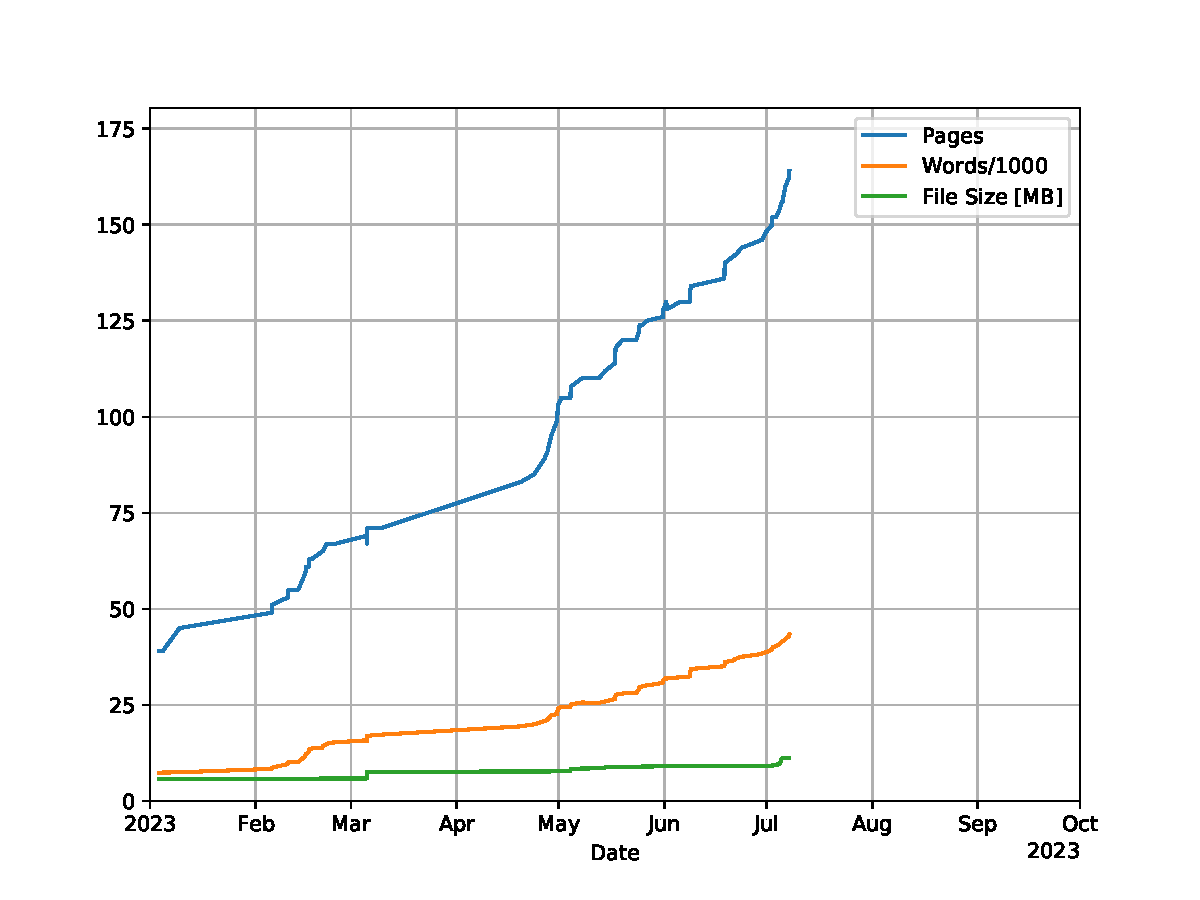
\includegraphics[width=\textwidth]{Figs/pdfstats_plot.pdf}
    \caption[]
    {Plot showing the development of this thesis, as a function of time.}
\end{figure}
\end{dedication}


% ************************** Thesis Acknowledgements **************************

\begin{acknowledgements}      

\textit{No man is an island, entire of itself; every man is a piece of the continent, a part of the main}\footnote{\textit{John Donne, Devotions upon Emergent Occasions}}. 
This is especially true in Experimental Particle Physics, which in recent decades has required large collaborations of people working together to explore the new frontiers. The making of this thesis is no different; I am deeply indebted to a great number of people who have helped me along the way. Here are some small words of thanks to you all.

To Armin Reichold, thank you so much for being my supervisor: always being there to ask the right questions about my work, and giving me advice about what to look at next. I made it through fighting SMELLIE thanks to your help. I've had so much fun doing research with you, learning so much thanks in part to your words to me: ``No black boxes''.

To Steve Biller and Jeff Tseng, your advice on matters of analysis, statistics, and computing have been invaluable. My work would be a shambles otherwise. Thank you also for building such a welcoming place to do Physics.

To Kim Proudfoot and Sue Geddes, who are the primary reason why the Particle Physics sub-department runs in any capacity. Also, to the IT Support staff; my work literally could not have been done without you guys keeping the interactive machines and internet connections working nicely. I'm sorry, Vip, for blocking the queue that time.

To the ever-growing family of colleagues and friends who I have had the pleasure of working in the SNO+ office with: Tereza, Iwan, Josh, Rafael, Cal, Gulliver, Abi, Jasmine, Qingyang, and Ellie. Special thanks to Josie for being an awesome thesis-writing buddy, and a brilliant friend. Also, to the elite strike squad of postdocs: Ed, Will, Ana Sofia, and Ben. I would be remiss in forgetting all the folks who have worked on SMELLIE, including Esther Turner and Jeff Lidgard. Jeff, thanks so much for being willing to fight through SMELLIE `integration hell' with me.

To Vic, Sierra, Caroline, Steph, Cindy, Matt, Mark, Aleksandra, Christine, and Ryan, thanks so much for making Sudbury so inviting whilst I was there; be it stuck underground without power, singing at Little Montreal, sliding on inflatables on Ramsey Lake, or getting stuck in Espanola. James and Rafael (again), it was great fun being housemates. Juliette, thanks for being my partner-in-crime as YM representatives: I hope your canoe is still okay.

To my friends outside the SNO+ cult, you are what makes life worth living: Eimear, Soniya, Ynyr, Ciaran, Niamh, Steph, Gwen, Sol, Ben, and so many others. Also, to everyone I've played with in Quadball (n\'{e}e Quidditch). Never Forget to be Awesome.

And finally, to my family: Mum, Dad, Joel, Ben, Leo, and Crumble. Thank you all for being so loving and fun, even after so many months in lockdown together. I would not be here without you. \textit{...All shall be well, and all shall be well, and all manner of thing shall be well.}\footnote{\textit{Julian of Norwich}}

\end{acknowledgements}

% ************************** Thesis Abstract *****************************
% Use `abstract' as an option in the document class to print only the titlepage and the abstract.
\begin{abstract}
This is where you write your abstract ...
\end{abstract}


% *********************** Adding TOC and List of Figures ***********************

\tableofcontents

\listoffigures

\listoftables

% \printnomenclature[space] space can be set as 2em between symbol and description
%\printnomenclature[3em]

% \printnomenclature

% ******************************** Main Matter *********************************
\mainmatter

%!TEX root = ../thesis.tex
%*******************************************************************************
%*********************************** First Chapter *****************************
%*******************************************************************************

\chapter{The Theory of Neutrino Physics}\label{chap:theory}  %Title of the First Chapter

%!TEX root = ../thesis.tex
%*******************************************************************************
%****************************** Second Chapter *********************************
%*******************************************************************************

\chapter{The SNO+ Detector}\label{chap:detector}
\section{Detector Geometry and Design}
\begin{itemize}
    \item Describe the SNO+ geometry at a high level: explain structure, and why certain design choices were made.
    \item Describe standard coordinate axis; note AV offset.
    \item Mention the main phases of SNO+, both past, present, and future.
\end{itemize}
\section{Detecting a Physics Event in SNO+: A Journey}
\begin{itemize}
    \item Begin the ``journey of a SNO+ Physics Event'' --- starting by explaining how a high-energy particle interacts with matter to generate Cherenkov and/or scintillation light. In both cases, optical wavelength light gets generated.
    \item Then, light propagates through the detector, possibly undergoing various physics processes: Rayleigh scattering, absorption, re-emission, refraction, and reflection.
    \item Light gets detected via the PMTs: explain how.
    \item Thus begins the DAQ chain. Signals reach the crates of electronics on deck and are processed. A ``sufficient signal'' leads to the triggering of the detector, which then enables for the saving of the event's information via the event builder.
\end{itemize}
\section{Calibrations and Detector Modelling}
\begin{itemize}
    \item I now describe how calibrations enable us to use the stored data for actual physics.
    \item Detector's state is continuously monitored via a number of systems for data quality purposes, including a human detector `shifter'. Mention use of run numbers. CHS and CSS ensure only ``good'' channels used in any analysis.
    \item First main set of calibrations are the ECAs and PCAs. These help us convert raw electronic signal information from PMTs into `calibrated' hit times and charges. PCAs performed via TELLIE and the Laserball.
    \item These initial calibrations allow for the first two passes of data processing. SMELLIE data comes from this part of the processing chain.
    \item In order to infer properties of an underlying physics event, an accurate model of the detector is needed. This requires two things: a set of calibration tools, and a piece of simulation software. The latter is RAT (explain briefly).
    \item Aims of remaining calibration tools are to obtain the optical parameters necessary for accurate modelling. Go through briefly all the calibration tools we have available: SMELLIE, AMELLIE, the Laserball, the AmBe and N16 sources, and in situ backgrounds.
    \item Using RAT once calibrated, event reconstruction can become possible. Briefly describe how energy, position, and time reconstruction works. Mention existence of direction fitting!
\end{itemize}
%!TEX root = ../thesis.tex
%*******************************************************************************
%****************************** Third Chapter **********************************
%*******************************************************************************
\chapter{Optical Scattering Theory}

% \include{Chapter4/chapter4}
\chapter{Simulating SMELLIE Events}\label{sect:beam_profiling}
Critical to extraction of scattering information from SMELLIE data is an accurate Monte Carlo (MC) simulation of the SMELLIE system. By modelling the laser light emission into the detector correctly, we can simulate how SMELLIE light will be impacted by changing scattering lengths in the detector. Because of the complexity of the optics of the optical fibres used to direct the laser light into the detector, a given SMELLIE event is simulated as a partially-collimated ``flash'' of visible photons emanating from the emission point of the fibre into the detector. This flash then requires a number of parameters to be correctly described. In particular:
\begin{itemize}
    \item \textbf{Fibre emission positions} were recorded during the installation of the fibres.
    \item \textbf{Wavelength and emission timing distributions} of light pulses were taken from measurements of the laser heads by their manufacturers~\cite{}, or by colleague Jeff Lidgard in the case of the SuperK wavelength distribution~\cite{}.
    \item \textbf{The ``pulse magnitude''}, defined as the mean number of photons simulated per event, is determined on a subrun-by-subrun basis, and is assumed to fluctuate as a Poisson distribution. 
    \item \textbf{The beam profiles}, which describe the angular emission distributions of each fibre, is the focus of this chapter. These are necessary because unlike scintillation light, the light emitted from SMELLIE fibres is not isotropic.
    \item \textbf{Nominal fibre emission directions} attempt to define the centre of the beam for a given fibre.
\end{itemize}

This chapter is split into three sections. Improvements to the existing simulation algorithm for the beam profiles are first made, and then the beam profiles themselves are updated. Finally, comparisons between data and simulation are made after the upgrades to investigate any remaining discrepancies.


\section{Improving the SMELLIE Generator Algorithm}
\subsection{Previous Attempts at SMELLIE Event Simulation}
Before we can determine the beam profiles, we must first decide how to specify them. Previous observations show that different fibres can have notably different beam profiles~\cite{majumdar_measurement_2015}, so we let each fibre's beam profiles be unique. We assume for now that a given fibre's beam profile is stable over time, and independent of the wavelength of light fired. A straightforward, na\"{i}ve approach to parameterising a beam profile would be as follows: specify some nominal fibre direction, corresponding to the direction light takes travelling from the fibre to the centre of the ``beamspot'' observed on the other side of the detector. Then, specify a 1D beam profile, corresponding to the probability density of firing a photon at a given polar angle $\alpha$ relative to the nominal direction. One might even assume this distribution is Gaussian. The distribution in azimuthal direction, $\phi$, is assumed to be uniform.

\begin{figure}
    \centering
    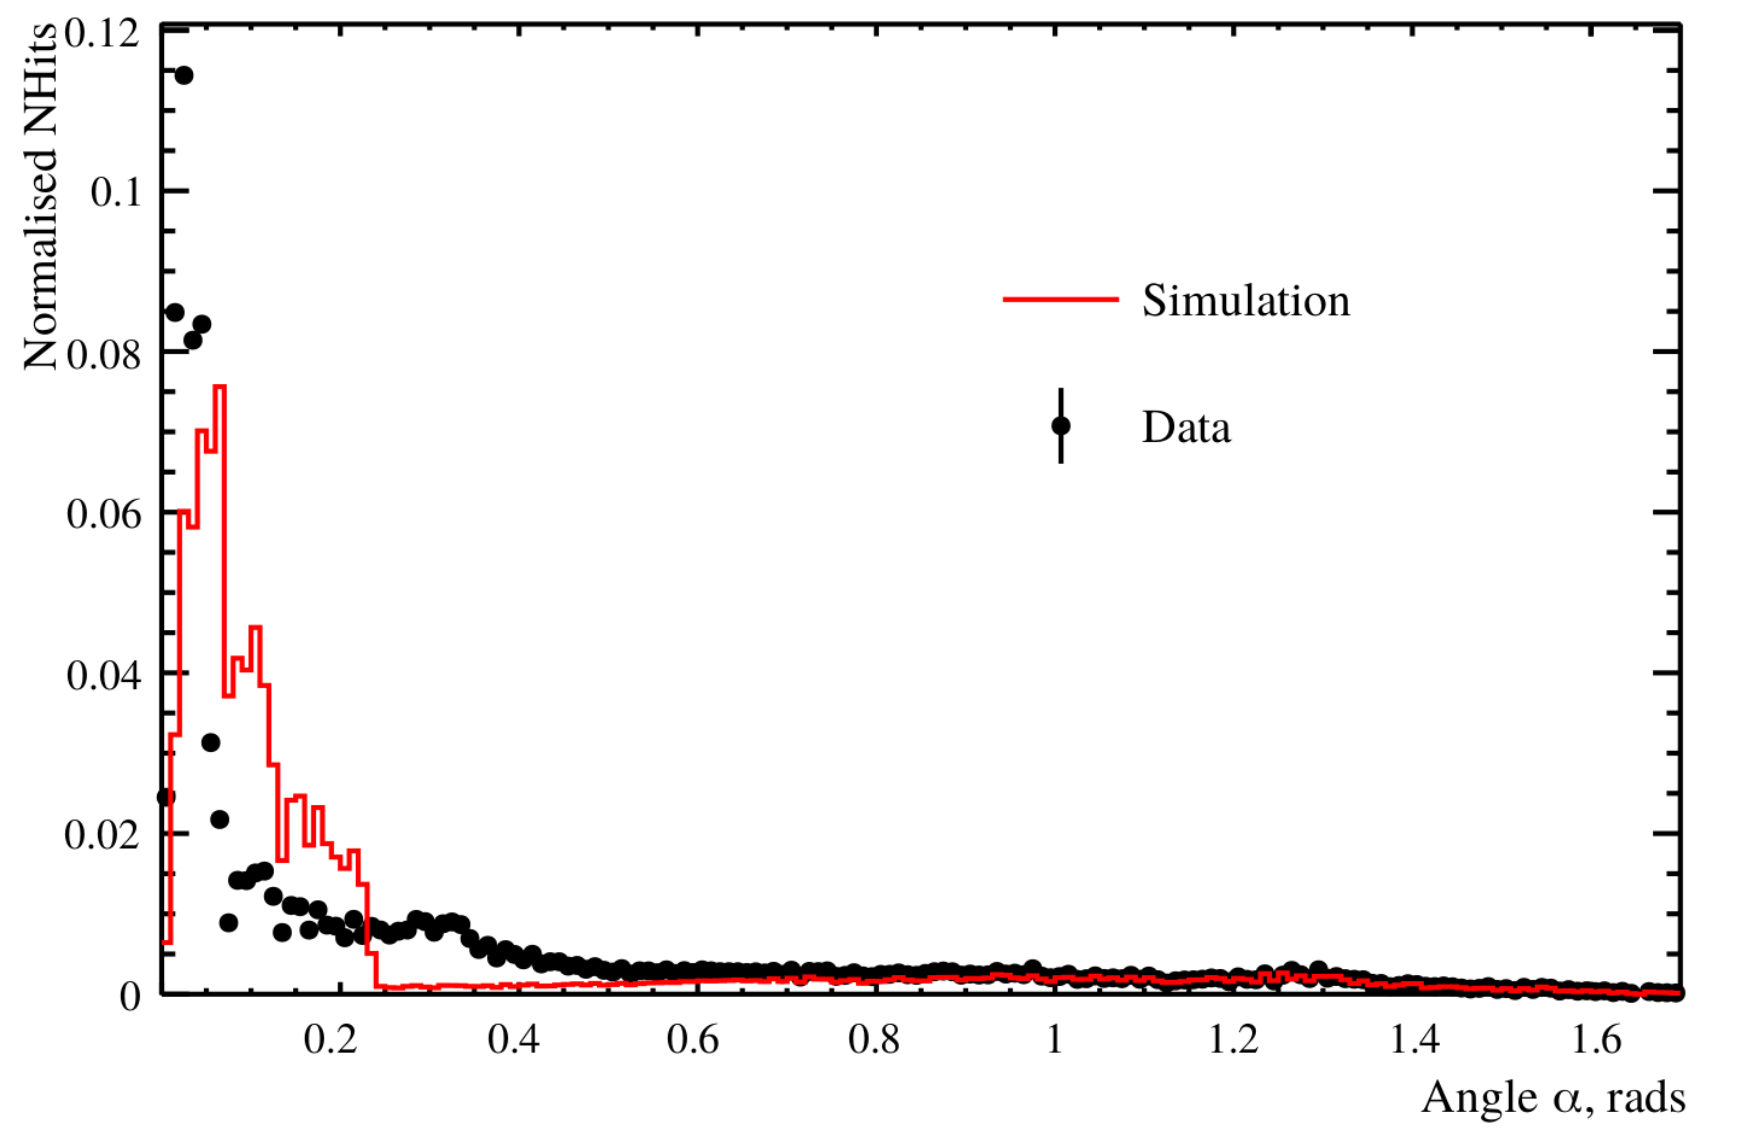
\includegraphics[width=0.7\textwidth]{5_SMELLIESimulation/images/1D_gen_plot.png}
    \caption{Comparison between a simulation of one of the fibres, made from the 1D beam profile generator (red), with the associated data subrun that was used to create that beam profile (in black). For both MC and data, what is plotted is the PDF of observed PMT hits, as a function of the $\alpha$ angle. Poissonian errors have been added to the data points, but are too small to see. Clearly, this 1D generator does not replicate the observed beam profile correctly. Figure taken from~\cite{turner_measurement_2022}.}
    \label{fig:1d_gen_plot}
\end{figure}

This 1D beam profile approach was used initially for SMELLIE, and remains in use for the other ELLIE sub-systems within SNO+. However, when SMELLIE data was taken in the water-phase of the experiment, simulations using these beam profiles failed to match them well at all - see figure~\ref{fig:1d_gen_plot} for an example. Not only was the distribution in $\alpha$ not Gaussian, a distinct speckle-pattern can be observed within the beamspot that is not uniform in $\phi$. This fact led to colleague Esther Turner building a SMELLIE generator that could handle 2D beam profiles: dependent on both $\alpha$ and $\phi$. The distribution was stored as a map from each inward-pointing PMT in the detector to a relative intensity value. This was chosen because the beam profile shapes were calibrated from existing SMELLIE data --- more on this in section~\ref{sect:new_beam_profiles}.

This original 2D generator then sampled the beam profile via a rejection sampling approach, outlined as follows:
\begin{enumerate}
    \item Propose a test direction $(\alpha, \phi)$, by generating $\phi$ uniformly in the interval $[0, 2\pi]$, and $\alpha$ according to some pre-determined Gaussian distribution, known as the Gaussian envelope.
    \item Given this test direction, calculate where a line following this direction from the fibre of interest will hit the PSUP on the other side of the detector. Find the 3 closest PMTs to that point.
    \item From those PMTs, obtain their relative intensity values from the beam profile mapping, and perform an interpolation based on how close each PMT is to the PSUP intersection point. This gives an interpolated relative intensity value for this test direction.
    \item Because we are sampling using the angular coordinates $(\alpha, \phi)$, differential area elements over this space of directions do not have the same size. We can correct for this fact by multiplying our interpolated relative intensity by $\sin{\alpha}$, which corresponds to the Jacobian of the direction-space.
    \item Calculate the value for the Gaussian envelope along this test direction.
    \item Throw a random number uniformly between 0 and the Gaussian envelope value. If the random number is less than the interpolated intensity, then this test direction is accepted, and a photon is generated with that direction. Otherwise, we reject the direction and try the whole process again.
\end{enumerate}

This generator certainly works, but has a key problem: efficiency. The 1D generator was able to generate a SMELLIE event (that is, to fully specify the starting parameters of all the photons emitted from a fibre) at a speed of $\sim\SI{1}{\milli\second}$. However, the 2D generator specified here could take upwards of $\sim\SI{50}{\second}$ \textit{per event} to generate. Because a typical SMELLIE analysis requires simulating many millions of events, the CPU time taken to perform this quickly became unfeasible. Fixing this generator speed problem was a high priority for the SMELLIE analysis.

\subsection{The new generator}\label{sect:new_gen}
On careful inspection of the existing 2D generator, the main reason for the slowness of the algorithm is the use of a rejection approach. Even with use of the Gaussian envelope, which was included to help with speed, the vast majority of proposed directions are never selected. Figure~\ref{fig:num_attempts} shows a histogram of number of attempts per event it took for a valid direction to be chosen for a representative SMELLIE simulation. Moreover, the calculations needing to be done for every proposed direction are relatively complex, notably trying to find the 3 nearest PMTs to some point on the PSUP.

\begin{figure}
    \centering
    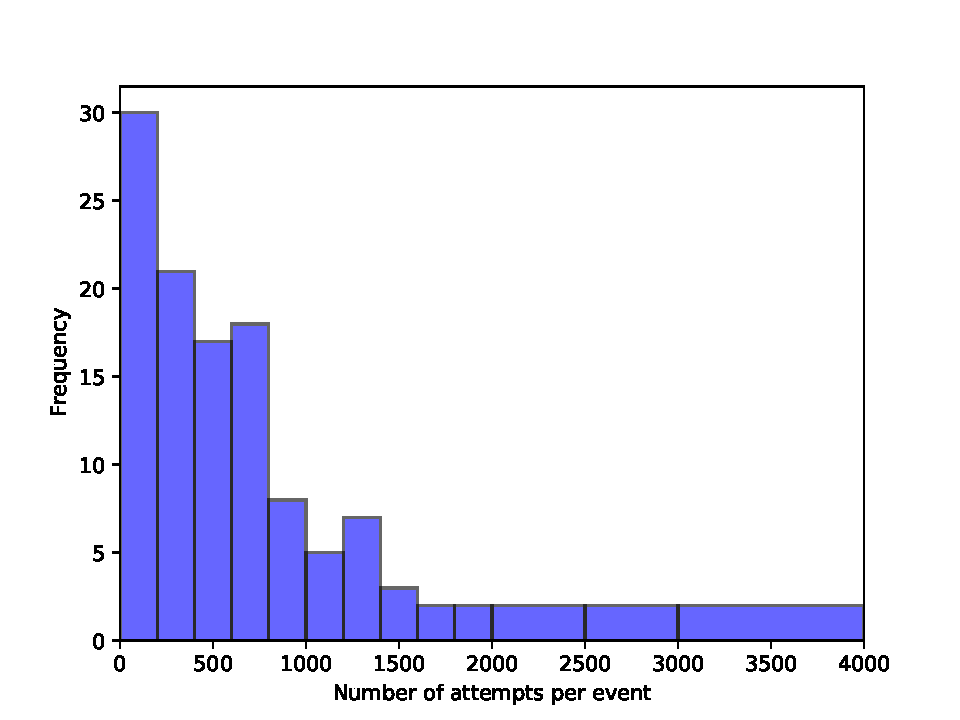
\includegraphics[width=0.7\textwidth]{5_SMELLIESimulation/images/2D_generator_num_attempts_nicer.pdf}
    \caption{Typical distribution of the number of attempts it takes for the existing 2D generator before the test direction gets accepted, per event.}
    \label{fig:num_attempts}
\end{figure}

A new 2D generator was built with these thoughts in mind. Firstly, the rejection method would no longer be used, given its inefficiency. We would also endeavour to try and ``pre-calculate'' as much as possible before run-time. Starting with the existing PMT relative intensity maps, we plot these in the 2D direction-space $(1-\cos\alpha, \phi)$: see Figure~\ref{fig:esther_beam_profile}. In a toy-MC simulation, \num{500000} directions are then thrown uniformly in this 2D space per fibre. For each direction, the same method of obtaining an interpolated intensity value from the nearest PMTs to the corresponding point on the PSUP as from the original 2D generator was performed, the only difference being that these calculations were done well before any actual SMELLIE simulation. Figure~\ref{fig:old_profile_interpolated_sample_plot} shows the interpolated intensities obtained for one fibre.

\begin{figure}
    \centering
    \begin{subfigure}{0.98\textwidth}
        \centering
        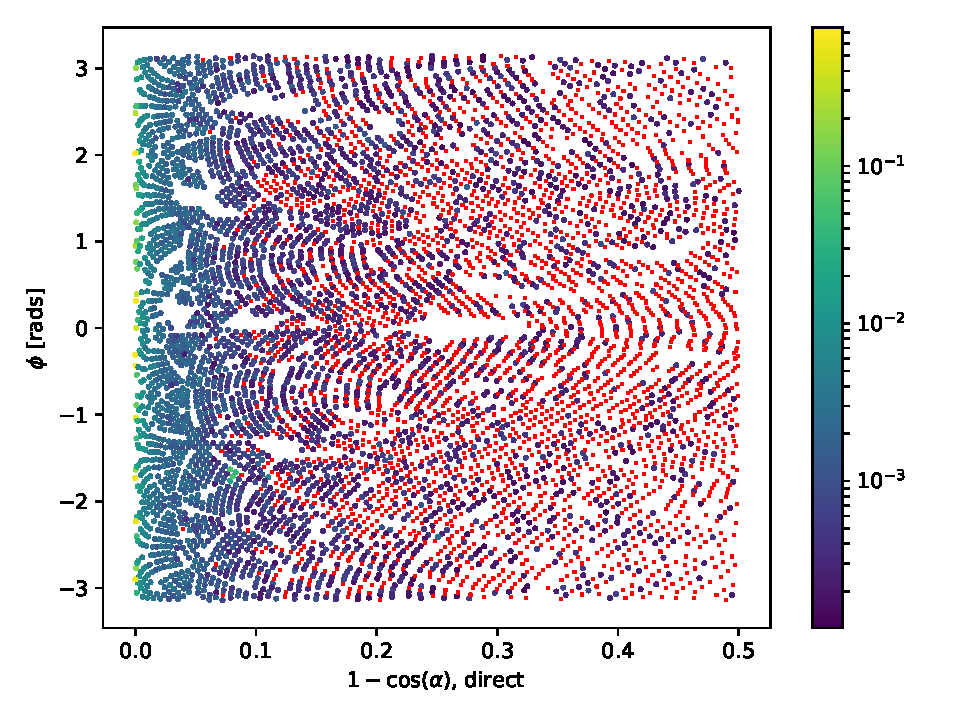
\includegraphics[width=0.8\textwidth]{5_SMELLIESimulation/images/flat_plot_r_FS055_beam_profile_original_6-18-13.pdf}
        \caption{PMT relative intensity map}
        \label{fig:esther_beam_profile}
    \end{subfigure}
    \begin{subfigure}{0.98\textwidth}
        \centering
        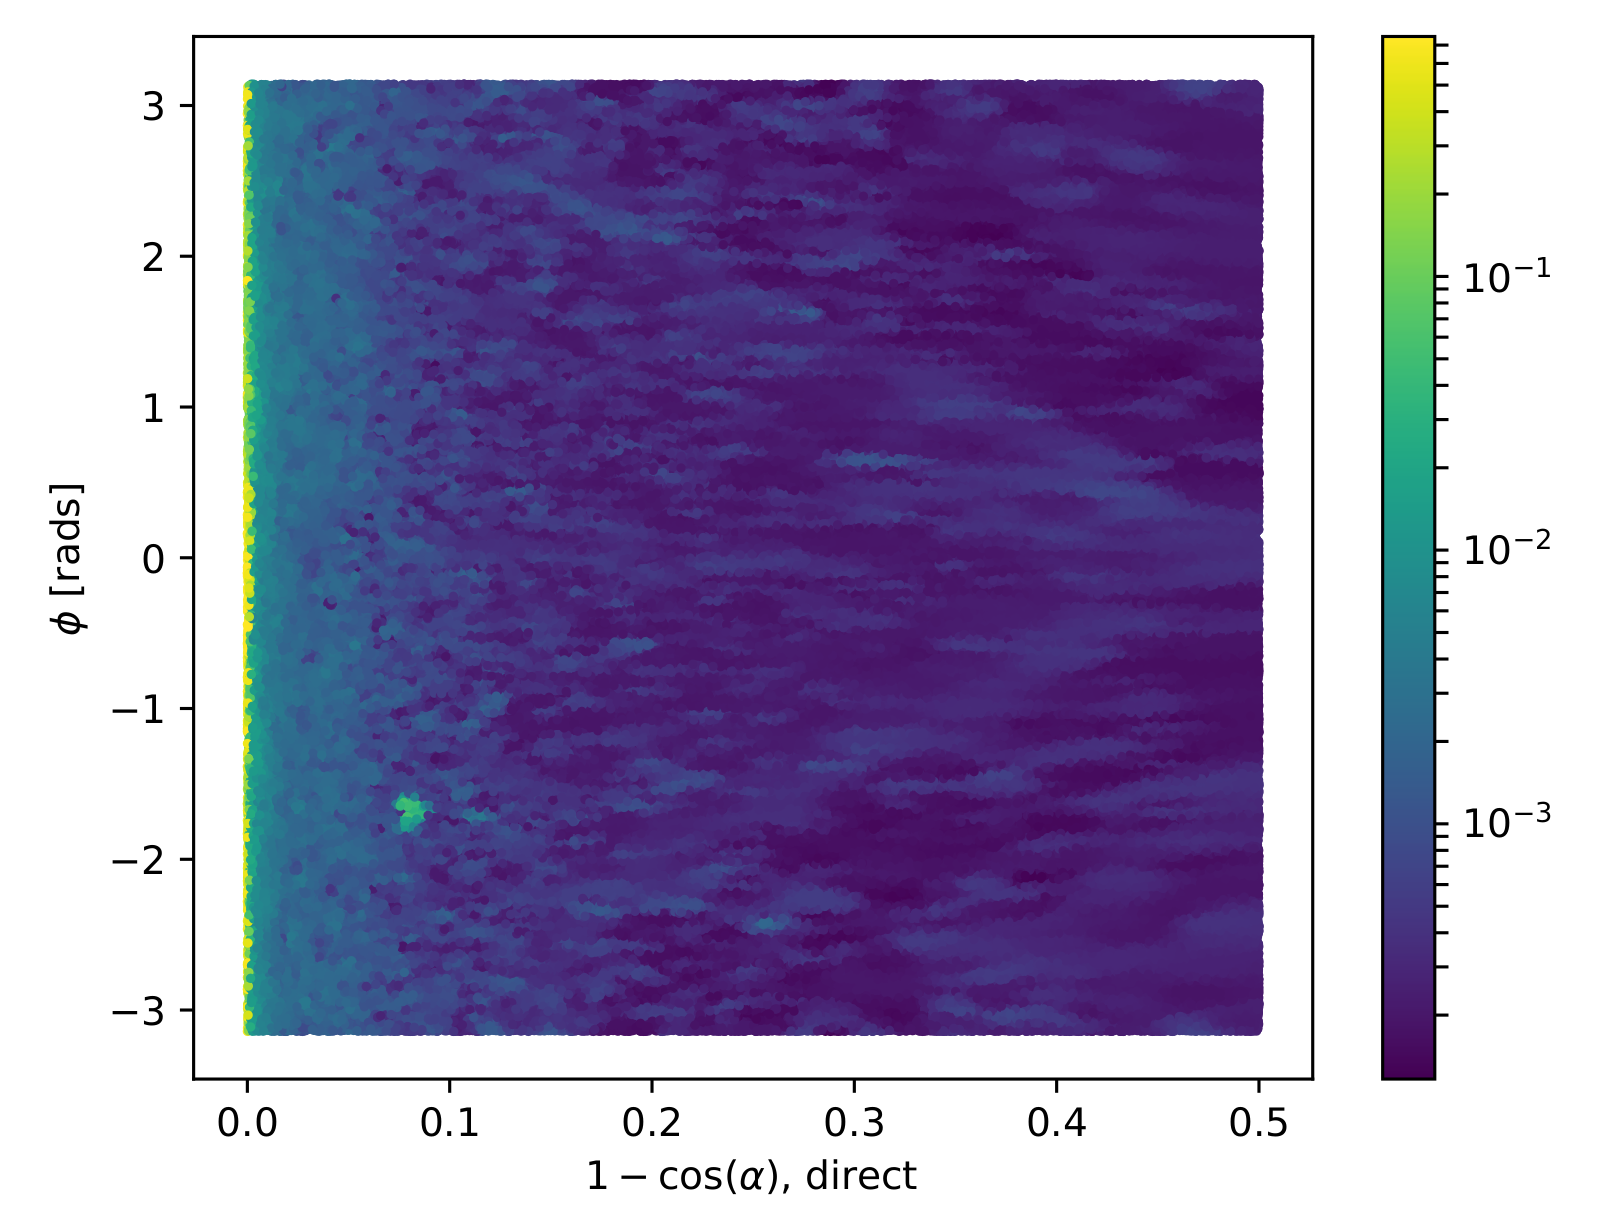
\includegraphics[width=0.8\textwidth]{5_SMELLIESimulation/images/polar_plot_FS055_MC_sampling_old_beam_profile.png}
        \caption{Interpolated intensity map}
        \label{fig:old_profile_interpolated_sample_plot}
    \end{subfigure}
    \caption{The first step in the new method for preparing the new generator. In (a), the relative intensities used for the existing beam profile of fibre labelled FS055 are shown for each PMT, the position on the plot indicating the location of that PMT in the fibre coordinates. The colour indicates the relative intensity; PMTs marked red have an intensity of zero. Figure (b) shows the result of throwing \num{500000} directions uniformly over this 2D space, the intensity of each point given by interpolating the intensities of nearby PMTs.}
    \label{fig:esther_beam_profile_and_interp}
\end{figure}

Following this, the sampled intensities were then binned into a 2D histogram, where the bin value corresponds to the sum of all intensities for all directions found within this bin. Choosing a sensible binning procedure is important: too few bins, and necessary information about the shape of the beam is lost, whilst too many bins can oversample the data and capture statistical artefacts in the sampling process instead of just the beam profile. As a balance, 15 bins were chosen along the $\phi$ direction, and 60 in $r=1-\cos\alpha$. This was chosen to ensure that a reasonable number of PMTs were located within each bin, lessening the impact of any statistical fluctuations. Although the bins in $\phi$ were chosen to have uniform width, this was decided to be not the case for the other axis, as there is far more important information near $r = 0$ (the beamspot). Instead, the width of the bins in $r$ were calculated so that roughly the same total probability was contained in each $r$-strip. By consequence, bins near the beamspot typically are of significantly smaller size than ones much further out. This allows us to both capture any rapid changes in intensity near the beamspot, where this matters greatly, and smooth out the very-low intensities seen at larger polar angles. One of these histograms can be seen in Figure~\ref{fig:hist_cdf_old_profile}: the large change in bin widths as a function of $r$ is clear. One can also see that near the beamspot notable dependence on the intensity as a function of $\phi$. The mysterious ``spot'' at $r = 0.08$, well out of the beamspot, is an indication that the underlying beam profile data being used requires improvement: more on this in section~\ref{sect:new_beam_profiles}.

\begin{figure}
    \centering
    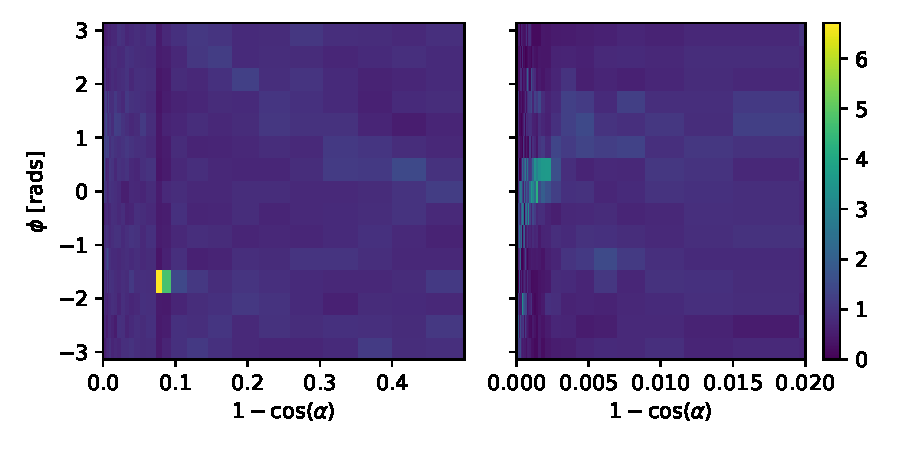
\includegraphics[width=\linewidth]{5_SMELLIESimulation/images/FS055_60_alpha_15_phi_hist.pdf}
    \caption{Histogram of interpolated intensities within the 2D direction-space. The left view shows the full histogram; the right is a zoomed-in version near the beamspot. Unlike the binning in $\phi$, the bin widths in $r$ are not at all uniform. Instead, they have been determined such that the area summed over a given ``strip" of bins of constant $r$ will be the same.}
    \label{fig:hist_cdf_old_profile}
\end{figure}

The Cumulative Density Function (CDF) of this intensity histogram as a function of bin was then produced, where the bins were ordered through a raster-scan: scanning first over $\phi$, and then $r$. The CDF was then normalised to 1 so that it was well-defined. It is this CDF object that is then loaded in and sampled from during event generation. To do this, an ``inverse-CDF'' approach was used, which has the major benefit over rejection sampling of always producing a valid direction for every sample made. The algorithm works as follows:

\begin{enumerate}
    \item Throw a random number uniformly in $[0,1]$.
    \item Perform a binary search to find the bin that has the largest CDF value below this random number.
    \item Look at the bin edges in $\phi$ of this selected bin: use linear interpolation of the random number to obtain a $\phi$ value located between these two $\phi$-values.
    \item Look at the selected bin's $r$-bin edges, and select a value of $r$ by throwing a second random number uniformly between the two edges. Convert this $r$ into a polar angle $\alpha$.
    \item The photon's direction is defined by the $(\alpha, \phi)$ chosen by this process. 
\end{enumerate}

Because of the relative simplicity of this algorithm compared to the previous 2D generator, the speed improvement was very large: generation now took $\sim\SI{1}{\milli\second}$ per SMELLIE event, a speed improvement of nearly $\num{50000}$. Event generation became as fast as it was when the 1D generator was being used. Furthermore, because of the approach taken, this major speed improvement comes at no sacrifice in accuracy. Figure~\ref{fig:data_generator_comp_new_profiles} shows a comparison of the average number of photoelectrons (npe) per event per PMT between water-phase SMELLIE data and simulations with both the old and new 2D generator. One can see clearly that both generators are as accurate as one another. Note that this plot uses the updated beam profiles as explained in the next section.

\begin{figure}
    \centering
    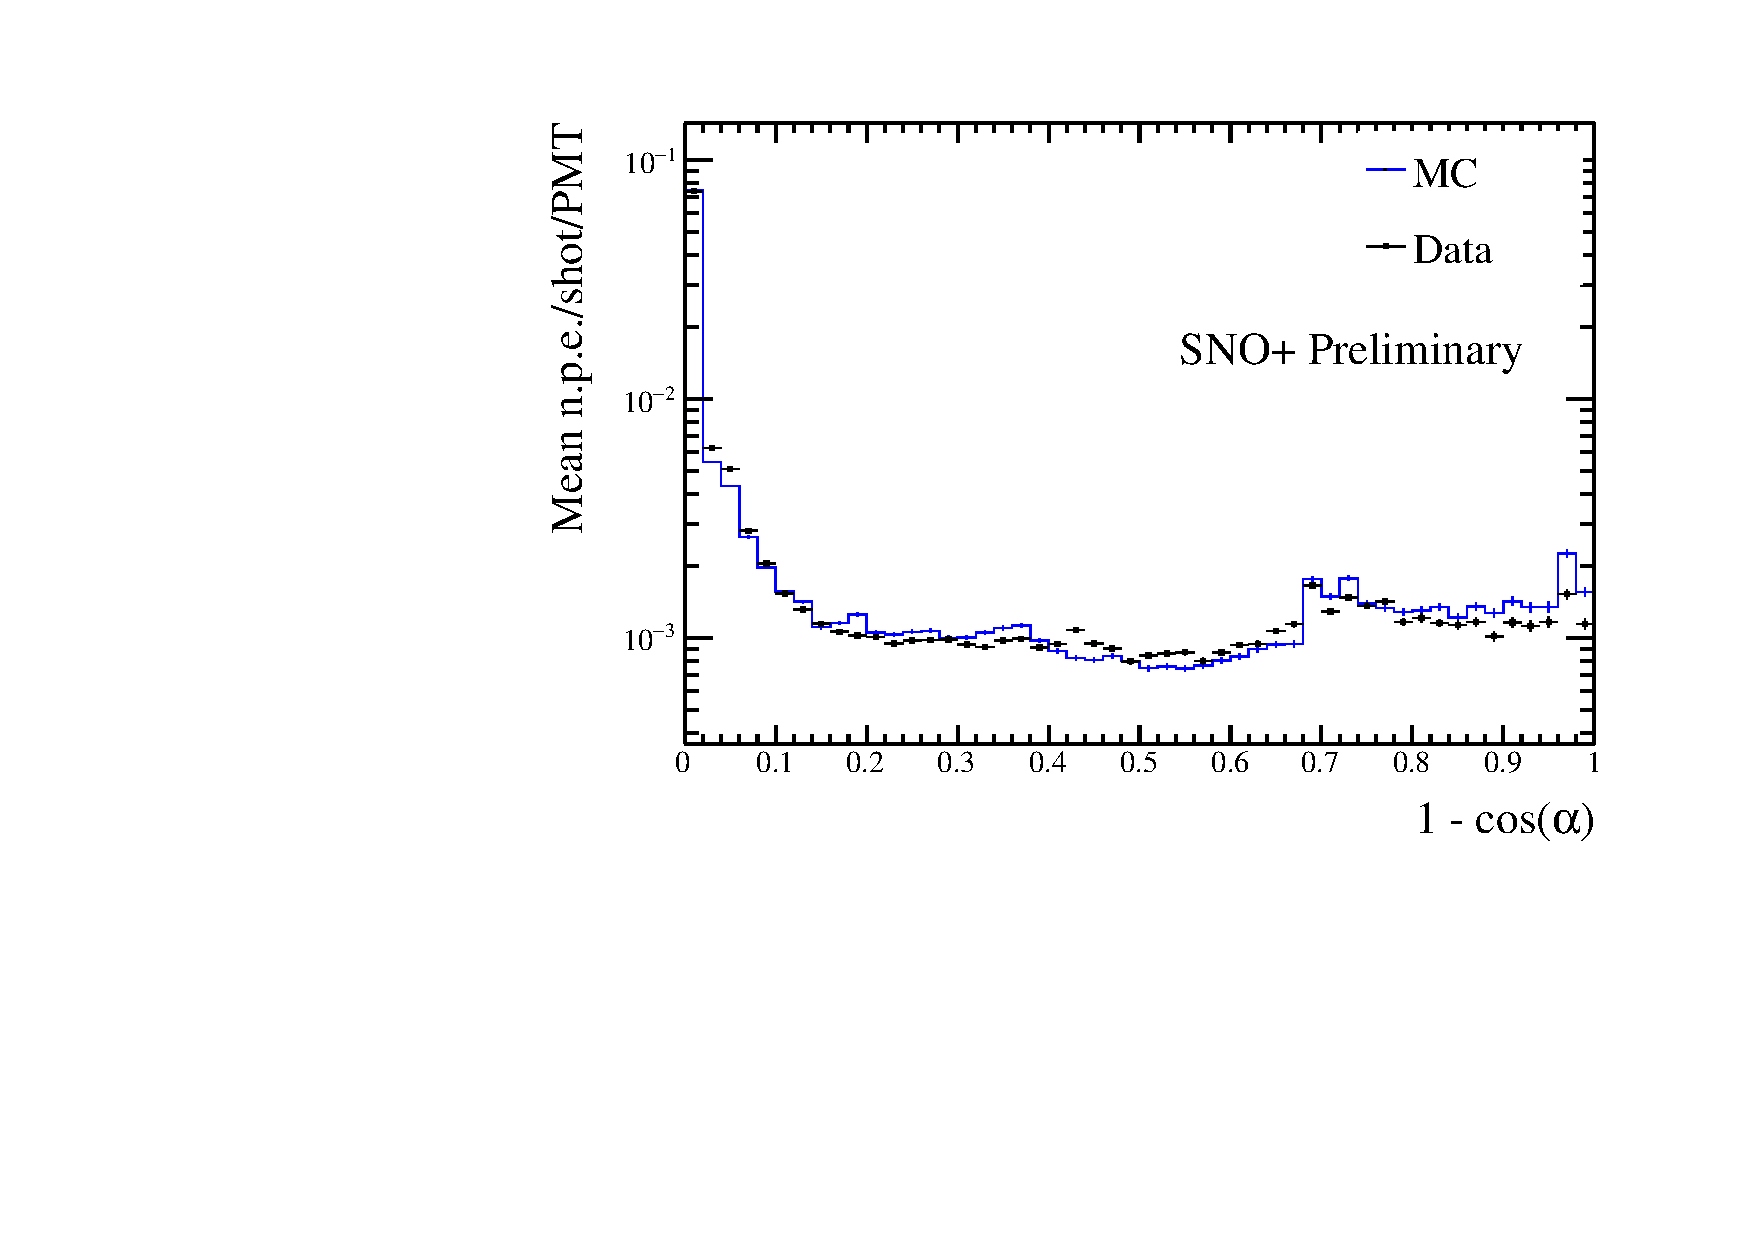
\includegraphics[width=\linewidth]{5_SMELLIESimulation/images/data_mc_comparison_npe_vs_r_114018_109_use_f.pdf}
    \caption{Comparison of water-phase data to MC generated using both the old and new 2D beam profile generator approaches, with the updated beam profiles. Both versions of the generator are consistent with one another, but the new generator is many times faster.}
    \label{fig:data_generator_comp_new_profiles}
\end{figure}

\subsection{Improving the beam profiles}\label{sect:new_beam_profiles}
Even with the new 2D profile generator, a problem remains: the simulation fails to reasonably recreate data, and much of this appears to be because of the poor beam profile data being used. The curious ``spot'' for one of the fibres was already noted in the previous section that doesn't seem to be physical, and more broadly at large angles for all the fibres there are large swathes of PMTs with an intensity of zero, providing little useful information about the beam shape. It was shown in~\cite{turner_measurement_2022} that with the old 2D generator, the systematic uncertainty on the beam profiles was the dominant source of error in the main SMELLIE analysis. To help improve this situation, it was decided to update the existing beam profiles.

These old beam profiles were originally determined by looking at SMELLIE data taken during the water-phase. Specifically, a ``medium''-intensity subrun with one of the lasers firing at a wavelength of \SI{495}{\nano\metre}, was chosen for each fibre. ``Medium''-intensity corresponds to firing the relevant laser at a set intensity determined during an earlier commissioning process, for which the maximum occupancy of PMT hits at that intensity, i.e. the proportion of hits per event, corresponded to roughly 80\%. This value was chosen as it allowed for high statistics in a relatively short run-time, but not so intense that the occupancy of any given PMT in the beamspot was 100\%. Because Rayleigh scattering is strongly-dependent on wavelength, the long wavelength of light was chosen so that impacts from this scattering were small in the data.

SNO+ PMTs are unable to distinguish the exact number of photoelectrons being generated. One is typically only able to know if a PMT has been triggered at all, by any number of photoelectrons. As a result, the occupancy of a PMT over a number of SMELLIE events, $o$, is a biased estimator of the mean number of photoelectrons generated, $\mu$. Assuming the number of photoelectrons generated in a given event follows Poisson statistics, the probability of generating $k$ photoelectrons is:

\begin{equation}
    P\left(k | \mu\right) = \frac{\mu^{k}e^{-\mu}}{k!}.
\end{equation}

The probability of observing a ``hit'' in a given PMT corresponds to generating at least one photoelectron:

\begin{equation}\label{eq:p_hit}
    P\left(\text{hit}| \mu\right) = P\left(k\geq 1 | \mu\right) = 1 - P\left(k = 0 | \mu\right) = 1 - e^{-\mu},
\end{equation}
which implies after rearrangement that one can determine the mean number of photoelectrons per event from the occupancy by:
\begin{equation}\label{eq:multihit_correction}
    \mu = \ln\left(1 - o\right).
\end{equation}
This is the reason why we want to avoid PMTs with occupancies of 100\%: they preclude one's ability to convert into a value for $\mu$ by looking at occupancy alone. We call this conversion from occupancy into npe the ``multi-hit correction''. The impact of this correction is typically small for most PMTs, but can become very significant in a fibre's beamspot.

Once the npe mapping from data was obtained, a correction was then made for the detector's optics: even ignoring a fibre's beam profile, we still expect certain PMTs to be illuminated more than others because of e.g. reflections off the AV, or the solid angle subtended by the PMT bucket opening. For each fibre, a simulation was made where the beam profile was set as isotropic, and the corresponding npe mapping obtained: this map held information about the detector optics only. The beam profile mapping was then derived by simply dividing each fibre's npe mapping from data to its associated isotropic MC npe map. It is these maps that were first used in section~\ref{sect:new_gen}.

\subsection{Combining beam profile datasets}
% \begin{center}
    \begin{table}
        \begin{tabular}{c p{6cm} p{6cm}}
            \hline
            Run Number & Run Type & Comments \\ \hline \hline
            \num{114018} & All PQ lasers; SuperK laser in \SIrange{400}{500}{\nano\metre} range & Only PQ495 laser and SuperK at \SI{495}{\nano\metre} is used \\
            \num{114023} & SuperK laser in \SIrange{500}{600}{\nano\metre} range & Part 1 of this wavelength range; crash occurred on last subrun, so that subrun is ignored \\
            \num{114034} & SuperK laser in \SIrange{500}{600}{\nano\metre} range & Part 2 of this wavelength range \\
            \hline
        \end{tabular}
        \caption{Water-phase runs used for new beam profiling.}
        \label{tab:runs_used}
    \end{table}
% \end{center}
Fortunately, much more SMELLIE data was taken during the water-phase than was used for the original beam-profiling analysis. This additional data can be combined with that which was already used to far better constrain the beam profiles. In particular, given the existing assumption that scattering effects are minimal above wavelengths of $\sim\SI{490}{\nano\metre}$, all data taken with wavelengths above this can also be used. The specific runs (and associated comments about their specifics) are described in Table~\ref{tab:runs_used}. Because high-intensity runs require a different analysis approach (PMTs with high occupancies must use charge, not occupancy, to  estimate npe), for this analysis we only considered subruns that used low or medium intensity set-points.

For each subrun $j$ of data per fibre, we look only at PMT hits for each PMT $i$ that has been identified as ``good'' for that subrun\footnote{Strictly speaking, a PMT's ``goodness'' is only determined on a run-by-run, not a subrun-by-subrun level, but this has no impact on the analysis.}, $i \in G_{j}$. $G_{j}$ here represents the set of good PMTs in subrun $j$. In particular, a ``good'' PMT must have valid electronic and timing calibrations, be at high voltage and masked into the detector's trigger system for that subrun. In addition, an angular cut of $\alpha < \SI{60}{\degree}$ was made to remove PMTs that are well outside any reasonable beam direction. To isolates the hits arriving directly from the fibre without reflecting, scattering, or being noise, a time cut was also made. Because what matters is the time relative to emission from the fibre, and the expected time-of-flight from fibre to different PMTs varies, a quantity known as the time residual was used. Starting with the calibrated hit time of a given PMT relative to the event's trigger time, $t_{hit}$, the expected time-of-flight $t_{TOF}$ from the fibre to the PMT was subtracted, estimated with the collaboration's ``Light Path Calculator''. Then, the emission time was also subtracted, $t_{emm}$, estimated by looking at the second-earliest value of $t_{hit}-t_{TOF}$ within the fibre's central beamspot, defined as the PMTs for which $\alpha<\ang{3}$. It was found that a ``loose'' time residual cut of $t_{res} \in [-10, +12] \si[]{\nano\second}$ was sufficient to remove the vast majority of non-direct light with little signal sacrifice. In the situation where a subrun with intensity was very small, it would not regularly have at least two hits in the beamspot, and so the time residuals calculated would not be valid for many events. To avoid this situation, a cut was made on any subruns with mean intensities below 9 within their beamspot. This value was chosen as it would mean a $2\sigma$ fluctuation downwards of $2\cdot\sqrt{9}=2\cdot3=\SI{6}{\npe}$ would still have more than the 2 hits necessary for timing reconstruction. One fibre, FS207, has no data subruns that satisfy this condition, and as such will have to be dealt with separately. For the time being, this fibre was ignored.

Extracting the underlying beam profiles from these data required some careful thought, especially because different subruns could have different intensities. Considering a PMT $i$ in subrun $j$, the mean number of photoelectrons generated per event in that PMT for that subrun, $\mu_{ij}$ can be decomposed as follows:

\begin{equation}\label{eq:mu_def}
    \mu_{ij} = I_{j}k_{i} = I_{j}b_{i}f_{i}.
\end{equation}
$I_{j}$ is the intensity of the subrun, i.e. the mean number of photons generated from the fibre in that subrun per event. $k_{i}$ is the probability that a given photon generated at the fibre source ends up generating a photoelectron in PMT $i$. This itself can be further split into two components: $b_{i}$, the probability that a given photon at the fibre source points in the direction of PMT $i$; and $f_{i}$, the probability that a given correctly-pointed photon actually makes it to the PMT and successfully generates a photoelectron. It is $b_{i}$ that is the actual beam profile we would like to measure.

Letting $p_{ij}$ be the probability of observing a hit for a given event on a given PMT, the probability of observing $m_{ij}$ hits out of $N_{j}$ events in the subrun will be binomially-distributed:
\begin{equation}
    P(m_{ij}| \mu_{ij}) = L(\mu_{ij} | m_{ij}) = \binom{N_{j}}{m_{ij}}p_{ij}^{m_{ij}}(1-p_{ij})^{N_{j}-m_{ij}} = \binom{N_{j}}{m_{ij}}\left(1-e^{-\mu_{ij}}\right)^{m_{ij}}e^{-\mu_{ij}(N_{j}-m_{ij})}.
\end{equation}
Here we have used equation~\ref{eq:p_hit}, and noted that this probability distribution in $m$ can be re-framed as a likelihood function for the parameter $\mu_{ij}$. Considering only a single subrun of data, the maximum likelihood estimate of the parameter $\mu_{ij}$ can be shown to be:
\begin{equation}
    \left<\mu_{ij}\right> = -\ln\left(1-\frac{m_{ij}}{N_{j}}\right) = \ln\left(1-o_{ij}\right) \qquad(m_{ij} \neq N_{j}),
\end{equation}
where $o_{ij}$ is just the occupancy of PMT $i$ in subrun $j$. This is just the multi-hit correction formula seen in equation~\ref{eq:multihit_correction}, which makes sense.

When looking at multiple subruns for the same fibre, the total likelihood function for a given PMT when considering all the data for a given fibre will be the product of the likelihoods from each dataset,
\begin{equation}
    L\left(\left\{I_{j}\right\}, k_{i} | \left\{m_{ij}\right\}\right) = \prod_{j} L(I_{j}, k_{i} | m_{ij}) = \prod_{j}\binom{N_{j}}{m_{ij}}\left(1-e^{-I_{j}k_{i}}\right)^{m_{ij}}e^{-I_{j}k_{i}(N_{j}-m_{ij})}.
\end{equation}
This leads to a log-likelihood distribution of
\begin{equation}
    \mathcal{L}\left(\left\{I_{j}\right\}, k_{i} | \left\{m_{ij}\right\}\right) = \sum_{j}\left[\ln\left(^{N_{j}}C_{m_{ij}}\right) + m_{ij}\ln\left(1 - e^{-I_{j}k_{i}}\right) - I_{j}k_{i}\left(N_{j} - m_{ij}\right)\right].
\end{equation}
Formally, one could combine the likelihoods of all the PMTs together, and by looking at the maximum likelihood estimates for each of the parameters measure the parameter values this way. However, the set of equations one obtains through this approach quickly become analytically intractable, because the PMTs are coupled by the intensity values $I_{j}$. Even a direct numerical approach would be liable to fail: for a given fibre there can be dozens of subruns, and many thousands of PMTs of relevance, so the dimensionality of the system of equations would be far too large.

Because of this, a different approach was taken. It is expected that in a subrun the total npe, summed over all good PMTs, should be proportional to the intensity value $I_{j}$. One must be careful about this construction --- different subruns can have different sets of good PMTs, so two subruns with identical $I_{j}$ values could have a larger summed npe merely because more PMTs were good in that subrun. To counter-act this effect, only PMTs that were classified as good in \textit{all} subruns being analysed for that fibre would be used for the npe summation. In other words, we use data from PMT $i$ for summing only if:
\begin{equation}
    i \in \mathcal{I} = \bigcap_{j}G_{j}.
\end{equation}
We can then define the summed npe for a given subrun as $S_{j} = \sum_{i\in\mathcal{I}}\text{npe}_{ij}$, and assert that $I_{j} = cS_{j}$. By finding a value proportional to $I_{j}$, there is now enough information to maximise the log-likelihood $\mathcal{L}\left(k_{i} | \left\{m_{ij}\right\}, \left\{I_{j}\right\}\right)$ with respect to $k_{i}$ for each PMT independently, and hence obtain estimates for these $k_{i}$ parameters.

Of course, what is actually wanted are the underlying $b_{i}$ values, not $k_{i}$. This is where isotropic simulations come in. For each run of data used, a matching isotropic MC was produced. As an example, a simulation for run \num{114023} contained \num{200000} events for each fibre using an isotropic beam profile, over the full wavelength range considered in this run, \SIrange{500}{600}{\nano\metre}, using the same run conditions as in data (which PMTs were at high voltage, etc.).

For each isotropic MC run, both $I_{j}^{MC}$ and $k_{i}^{MC}$ were calculated via the method described above. Because the simulations were isotropic, the underlying value for $b_{i}$ was constant across all the PMTs, and so $ak_{i}^{MC} = f_{i}$. By doing some rearranging of equation~\ref{eq:mu_def}, we find that:
\begin{equation}
    \mu_{ij} = I_{j}b_{i}f_{i} = cS_{j}b_{i}ak_{i}^{MC} = (acb_{i})S_{j}k_{i}^{MC}.
\end{equation}
As a result of this, given the set $\left\{S_{j}\right\}$ and $k_{i}^{MC}$, one can maximise the log-likelihood $\mathcal{L}$ with respect to $b'_{i} = acb_{i}$ numerically, to obtain the maximum likelihood estimate of $b'_{i}$. Because $a$ and $c$ were global constants of proportionality, they would become irrelevant as soon as the beam profile was normalised in the CDF-creation process outlined in~\ref{sect:new_gen}.

Figure~\ref{fig:likelihood_scan} shows the shape of this log-likelihood distribution for a particular PMT when considering fibre FS007's beam profile. One can see how individual subruns provide much more information when combined than if one looked at a single subrun alone.

\begin{figure}
    \centering
    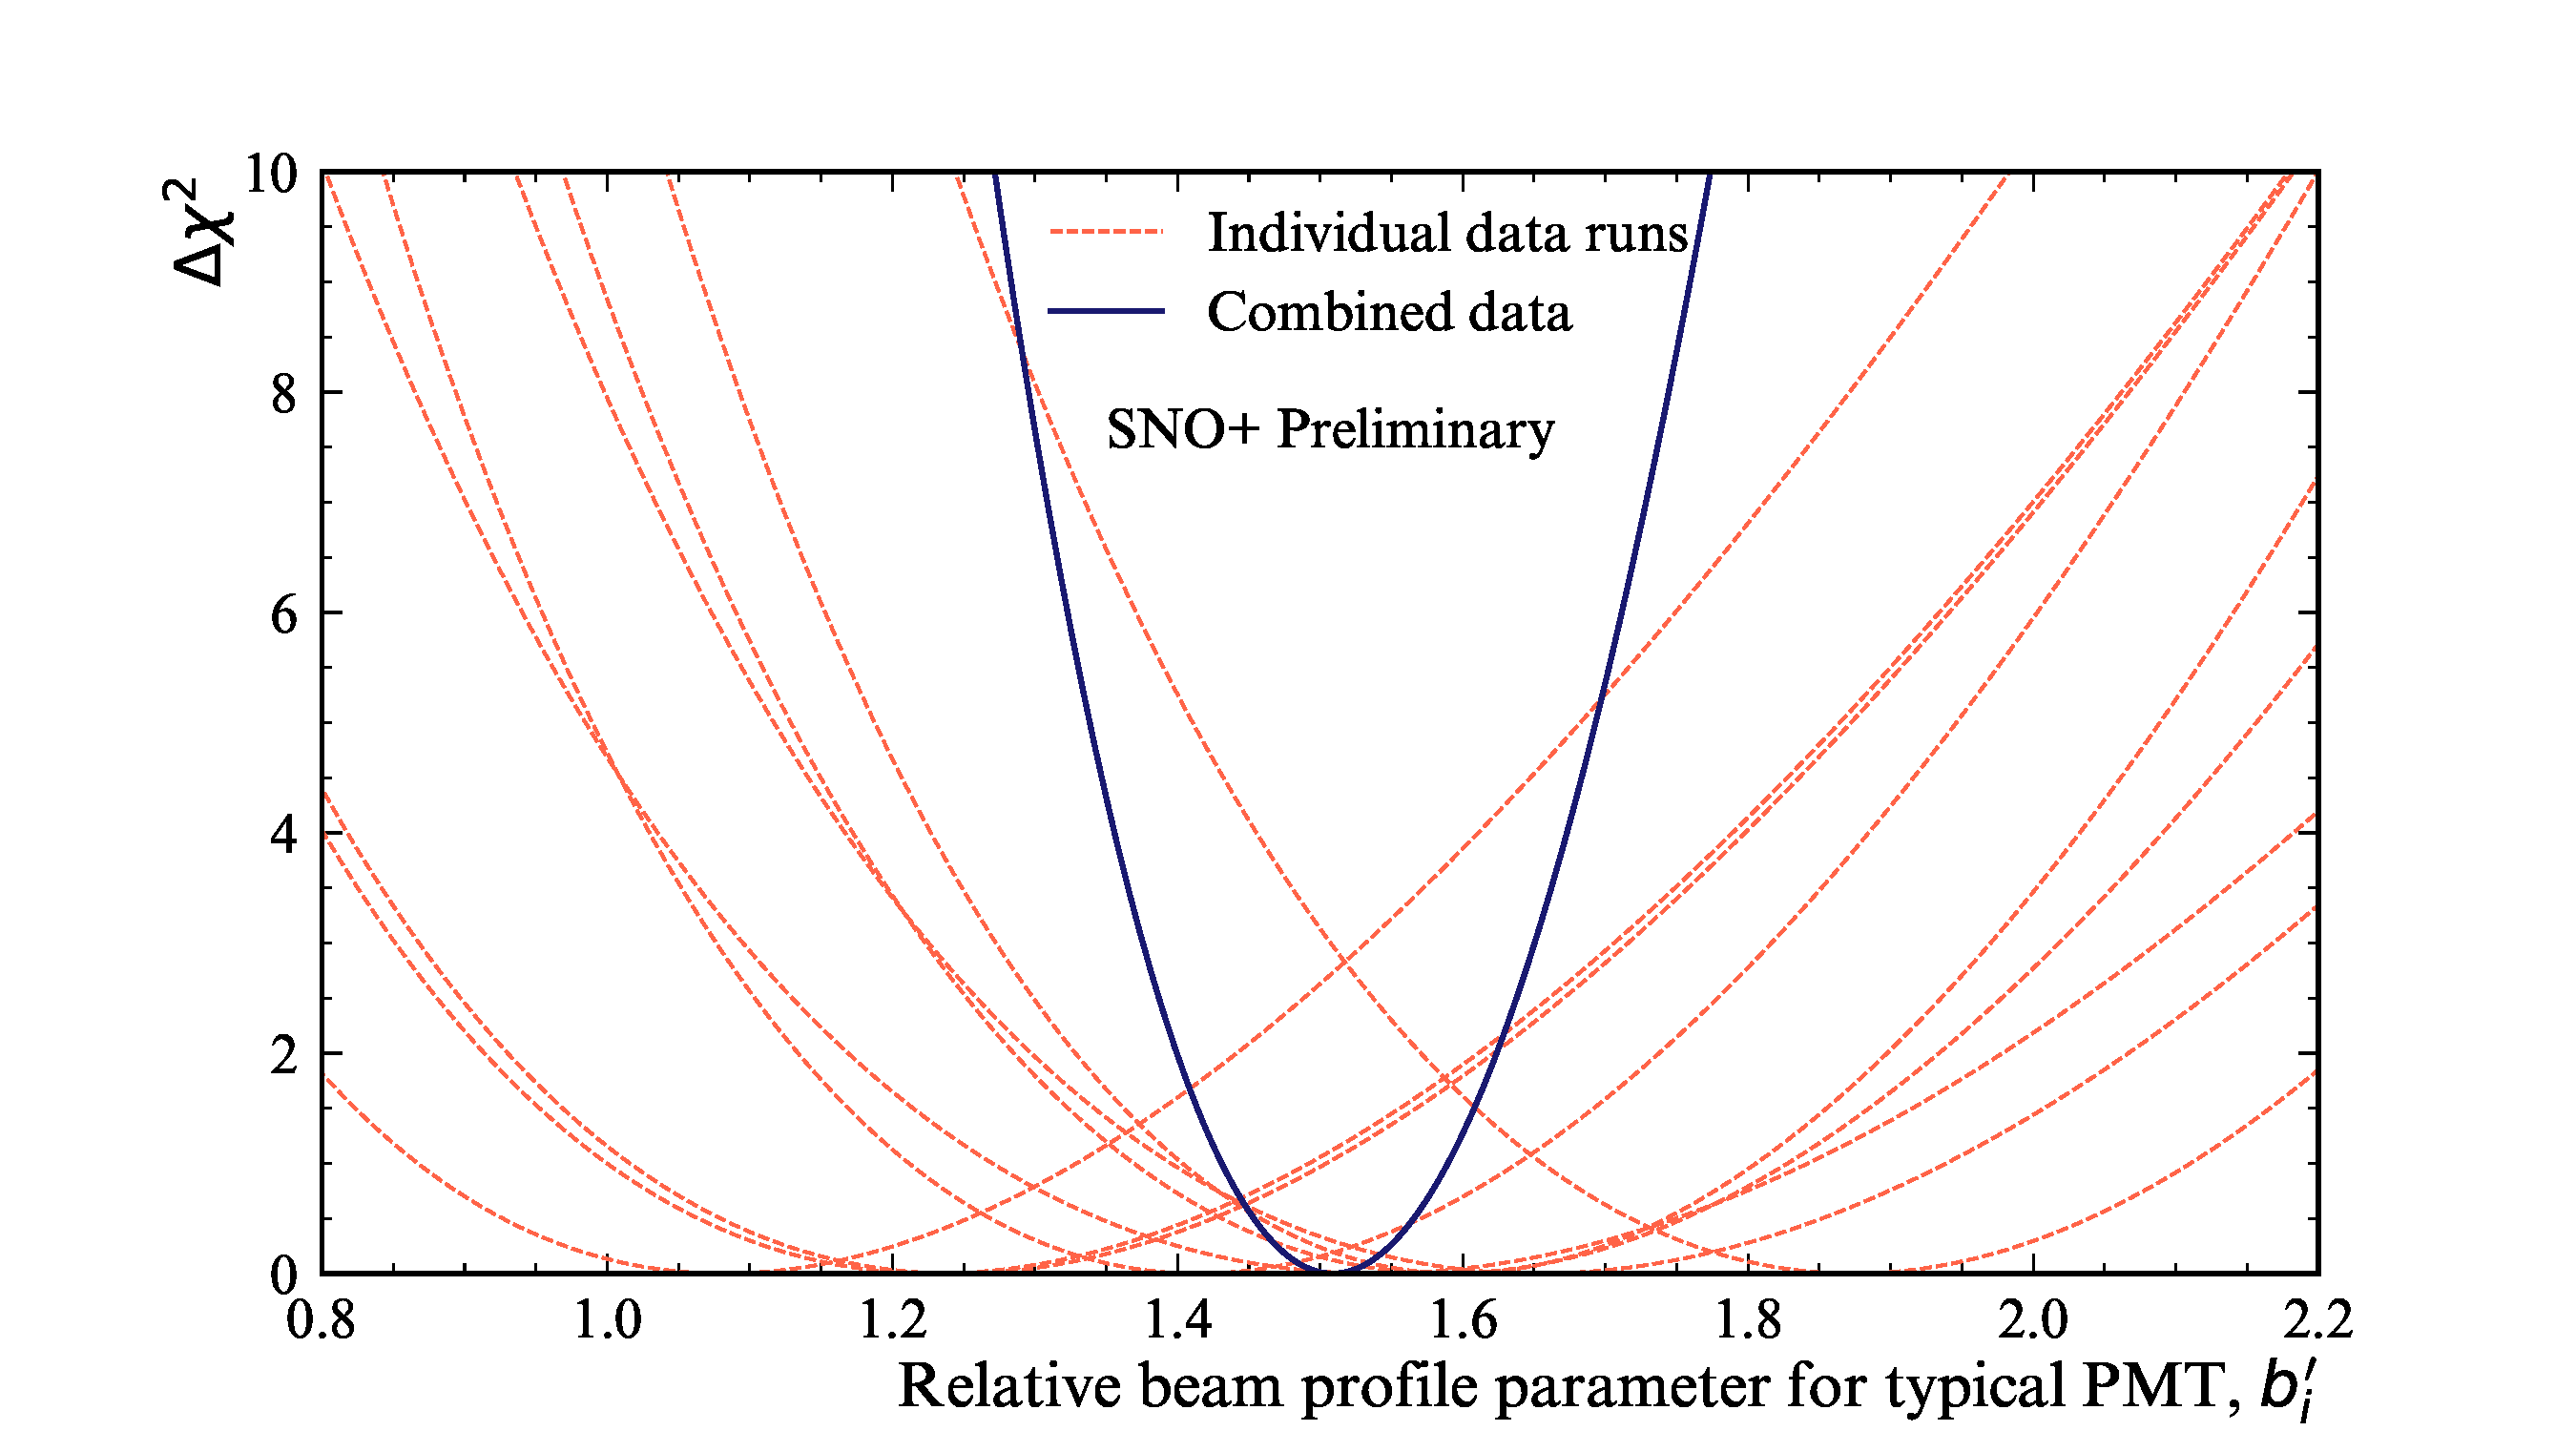
\includegraphics[width=0.8\linewidth]{5_SMELLIESimulation/images/example_likelihood_distribution_pmt_inc_all_subruns_proper_formatting.pdf}
    \caption{Plot of $\Delta\chi^2\simeq X_{i}$, twice the negative log-likelihood ratio, for both single subruns of a typical PMT, and when all relevant subruns are combined.}
    \label{fig:likelihood_scan}
\end{figure}

Another benefit of using this log-likelihood approach is that the resulting distribution's shape can be used for uncertainty estimation. In almost all cases, Wilks Theorem~\cite{wilks_large-sample_1938} allows us to produce $1 \sigma$ confidence intervals about the maximum likelihood estimate for $b'_{i}$, $\left<b'_{i}\right>$, because $$X(b'_{i}) = -2\left[\mathcal{L}\left(b'_{i}\right) - \mathcal{L}\left(\left<b'_{i}\right>\right)\right]$$ approximates a $\chi^2$-distribution. As a result, the error bounds on our parameter estimate are given by when $X = 1$. The fact that the shape of $X$ can be well-approximated by a quadratic in the region near $X = 0$ indicates the validity of Wilks' Theorem being used here.

Only a couple of exceptions to this approach of parameter estimation are possible. In the case where $m_{ij} = N_{j}$, i.e. a PMT has 100\% occupancy, no maximum likelihood estimate exists: we need not worry about this, as subruns where this occurs have not been used. On the other end, however, there are some PMTs for certain fibres where after all subruns of data have been included, there remains no hits. In this scenario, one can show that the log-likelihood becomes linear in the beam profile parameter:
\begin{equation}
    \mathcal{L}\left(b'_{i}|\left\{m_{ij}=0\right\}\right) = b'_{i}k_{i}^{MC}\cdot\sum_{j}\left[I_{j}N_{j}\right].
\end{equation}
This scenario is very much reminiscent of rare-decay searches, and a similar approach can be used. A $1 \sigma$ upper limit on the possible value for $b'_{i}$ can be analytically-calculated to be:
\begin{equation}
    b'_{i,ulim} = -\frac{k_{i}^{MC}\sum_{j}\left[I_{j}N_{j}\right]}{\ln\left[1 - \operatorname{erf}\left(1/\sqrt{2}\right)\right]},
\end{equation}
where $\operatorname{erf}(x)$ is the error function.

\subsection{Results \& Discussion}\label{sect:results}
Figure~\ref{fig:updated_beam_profile} shows the impact of using additional subruns of data on a typical beam profile. One can clearly see the great reduction in the number of PMTs with no hits in data. That many more data sets were included allowed for the major increase in dynamic range available for measuring these $b'_{i}$ values. One can also note that by including additional data the curious spot that was seen in the old beam profile our at $r\approx0.08$ has gone, further indicating that it was an artefact of that single data set.
\begin{figure}
    \centering
    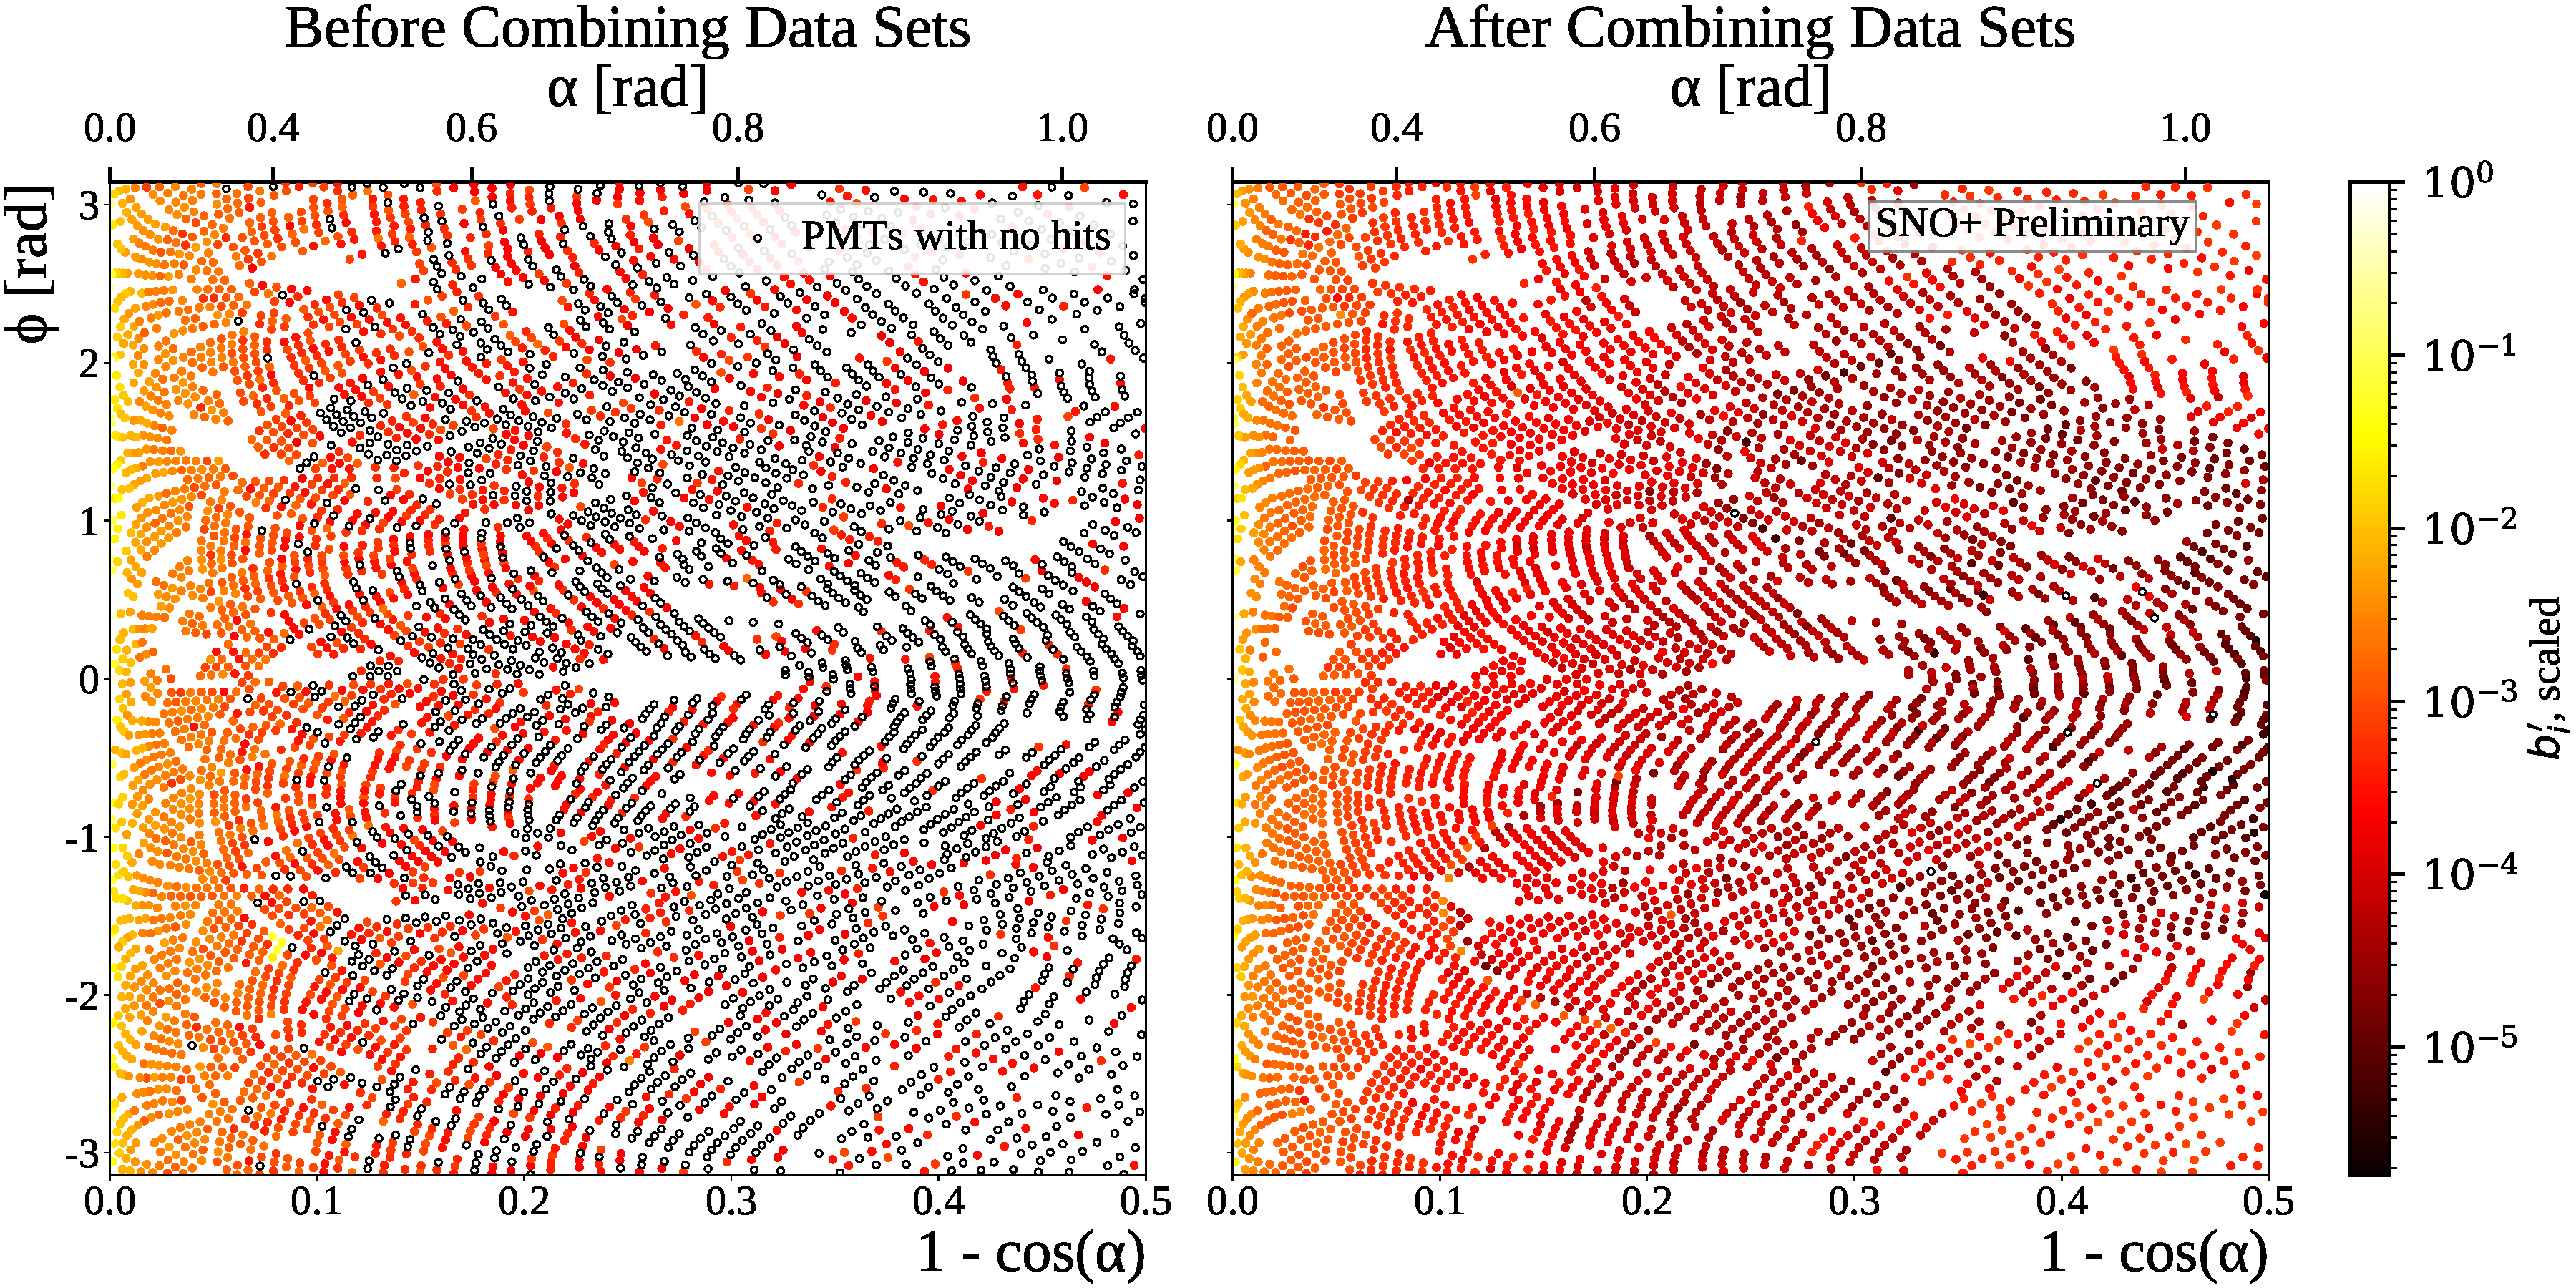
\includegraphics[width=0.8\textwidth]{5_SMELLIESimulation/images/flat_plot_r_comparison_FS055_old_vs_new_empty_circles.pdf}
    \caption{Comparison between old and updated beam profiles for fibre FS055, after combining multiple data sets. Once again, the relative intensities ($b'_{i}$) for each PMT are given by the colour of each point, the position of each plotted in the 2D $(r,\phi)$-space. The relative intensities have been both scaled here so that the largest value equals 1. Hollowed-out points are PMTs that, even after all relevant subruns have been combined, have no PMT hits.}
    \label{fig:updated_beam_profile}
\end{figure}

Further details can be gathered from the interpolated intensity maps, one of which can be seen in figure~\ref{fig:updated_beam_profile_sampling}. There are two curious stand-out features that can be seen here: firstly, there are multiple distinct parabolic arcs. These correspond to the shadows of the ropes that hold up/down the AV. More precisely, they are the mismodelling of those shadows --- if the shadows were in the right place in the isotropic MC, then they would correctly cancel out any decreased intensity seen in the data of shadowed PMTs. These shadows could be mismodelled either because the positions of the ropes in the MC are in the wrong place, or the fibre's emission position is wrong. Note that any mismodelling of the fibre's nominal emission direction has no impact on this shadowing problem, as changing that direction merely causes a change of basis in the $(r,\phi)$-space. The latter possibility of incorrect fibre positions are more likely, and in fact these arcs in the beam profiles could be used as an effective way to correct for this problem.

\begin{figure}
    \centering
    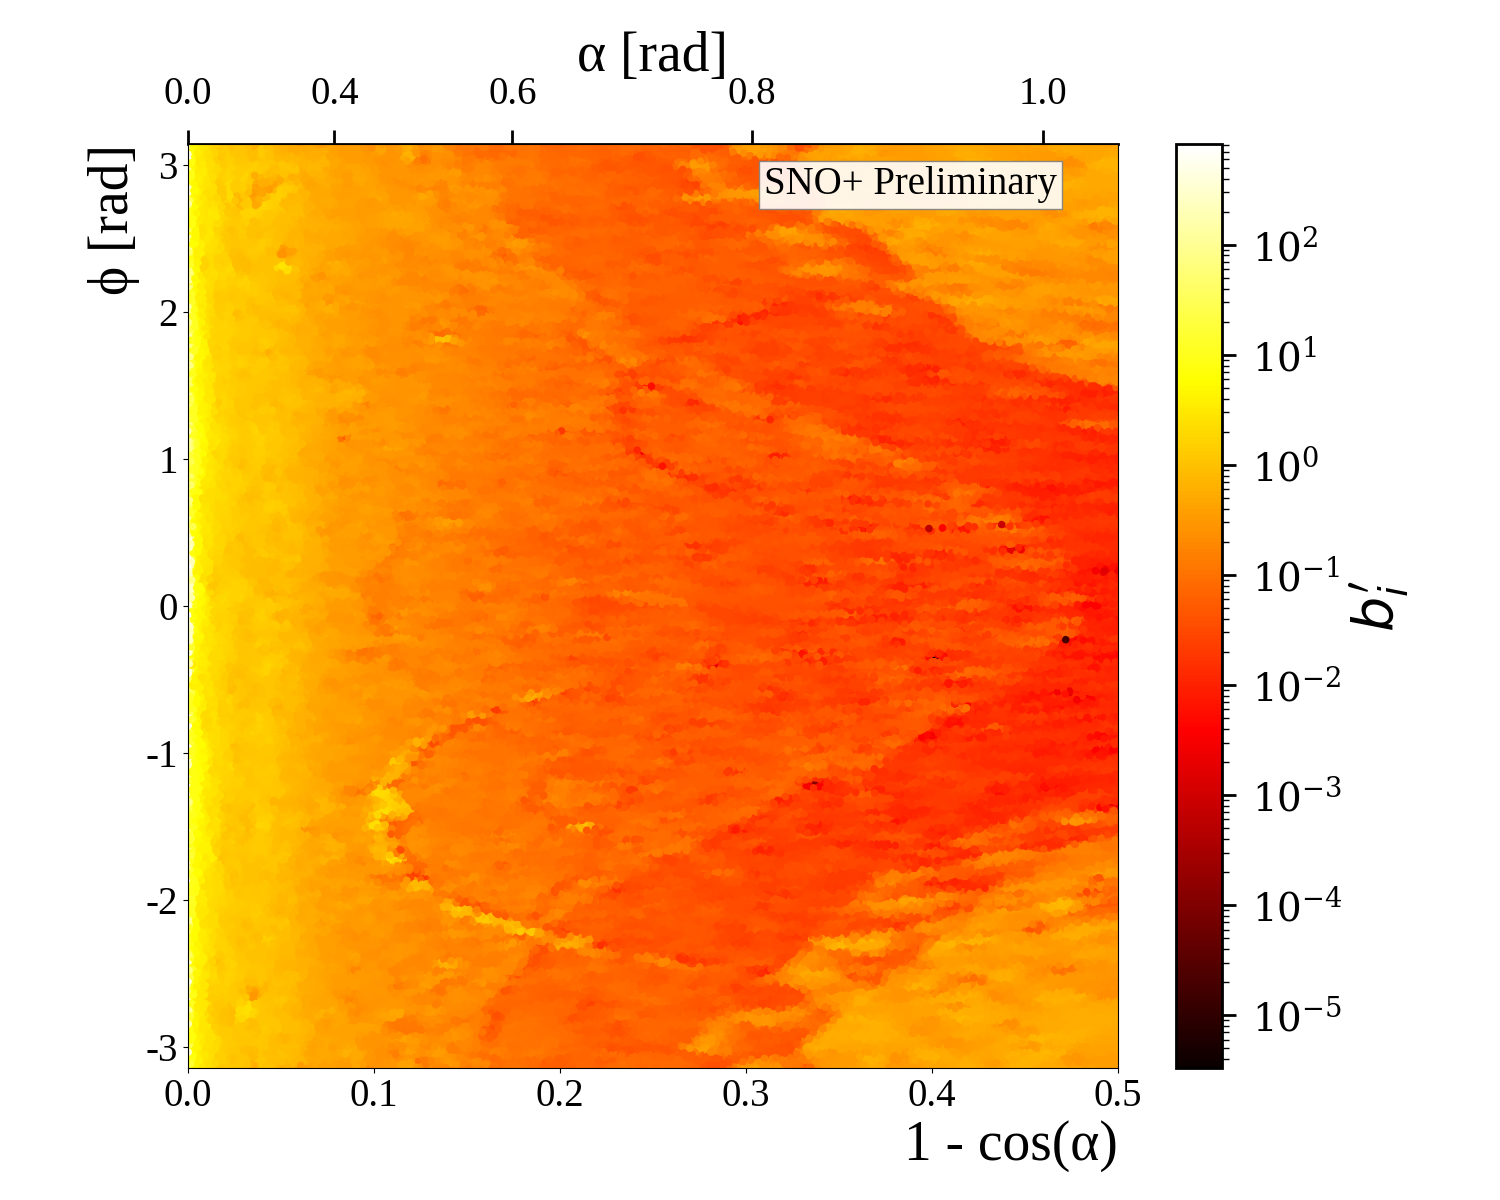
\includegraphics[width=0.8\textwidth]{5_SMELLIESimulation/images/flat_plot_r_FS055_500k_interpolated_beam_profile_full_formatting.png}
    \caption{Interpolated intensity map for the new updated beam profile of fibre FS055. The misalignment of rope shadows and AV effects, can both be seen.}
    \label{fig:updated_beam_profile_sampling}
\end{figure}
The second distinctive feature of this intensity map is the large band of lower intensity varying between $r\approx0.2-0.5$, followed by larger intensity out at large $r$ values. This feature comes from light reflecting off the AV surface, or internally-reflecting. The reason for this band's functional dependence on $\phi$ is that this particular fibre, FS055, has a nominal fibre direction $\sim\ang{10}$ from pointing radially-towards the detector's centre. This feature appears in the updated beam profiles of all fibres, but its shape depends on the particular fibre's direction --- for fibres pointing directly towards the detector's centre, there is little $\phi$-dependence observed. Like the ropes, this feature must come from some form of mismodelling of the optics of the AV. A de-facto shadowing of PMTs in line with tangents from the AV surface which intersect the fibre position is to be expected. One also expects PMTs at polar angles larger than this to have their observed intensities boosted from reflected light off the AV. However, the discontinuities seen in the beam profiles indicate that for whatever reason this effect has been over-emphasised in the simulation.

There is a further phenomenon that can be seen, by comparing beam profile values obtained from a single subrun to the updated combined beam profile. This can be done by calculating the residuals corresponding to the single subrun, relative to the combined data set. The residual is negative if the combined data sets have a $b'_{i}$ below the equivalent for a given single subrun; that is, the combined model underestimates this subrun for that PMT.

This information was plotted for two different subruns from the same fibre, seen in figure~\ref{fig:llr}. One subrun was the same one used by Esther Turner for the original 2D beam profiling, with a wavelength of \SI{495}{\nano\metre}; the latter was at the longer wavelength of \SI{595}{\nano\metre}. For both subruns, most PMTs are seen to have intensities well-modelled by the combined model. However, their appears to be a significant amount of mismodelling within the beamspot. There also appears to be some systematic shift between data and model at somewhat larger polar angles. Moreover, this mismodelling seems not to be merely random, but a function of wavelength: at shorter wavelengths the beamspot tends towards being overestimated and then underestimated at larger values of $\alpha$. At longer wavelengths, the beamspot becomes underestimated, with larger angles getting overestimated. This indicates that there appears to be a wavelength-dependence on the beam profiles, contradicting one of the main assumptions which we used to combine the water-phase data in the first place!
\begin{figure}
    \centering
    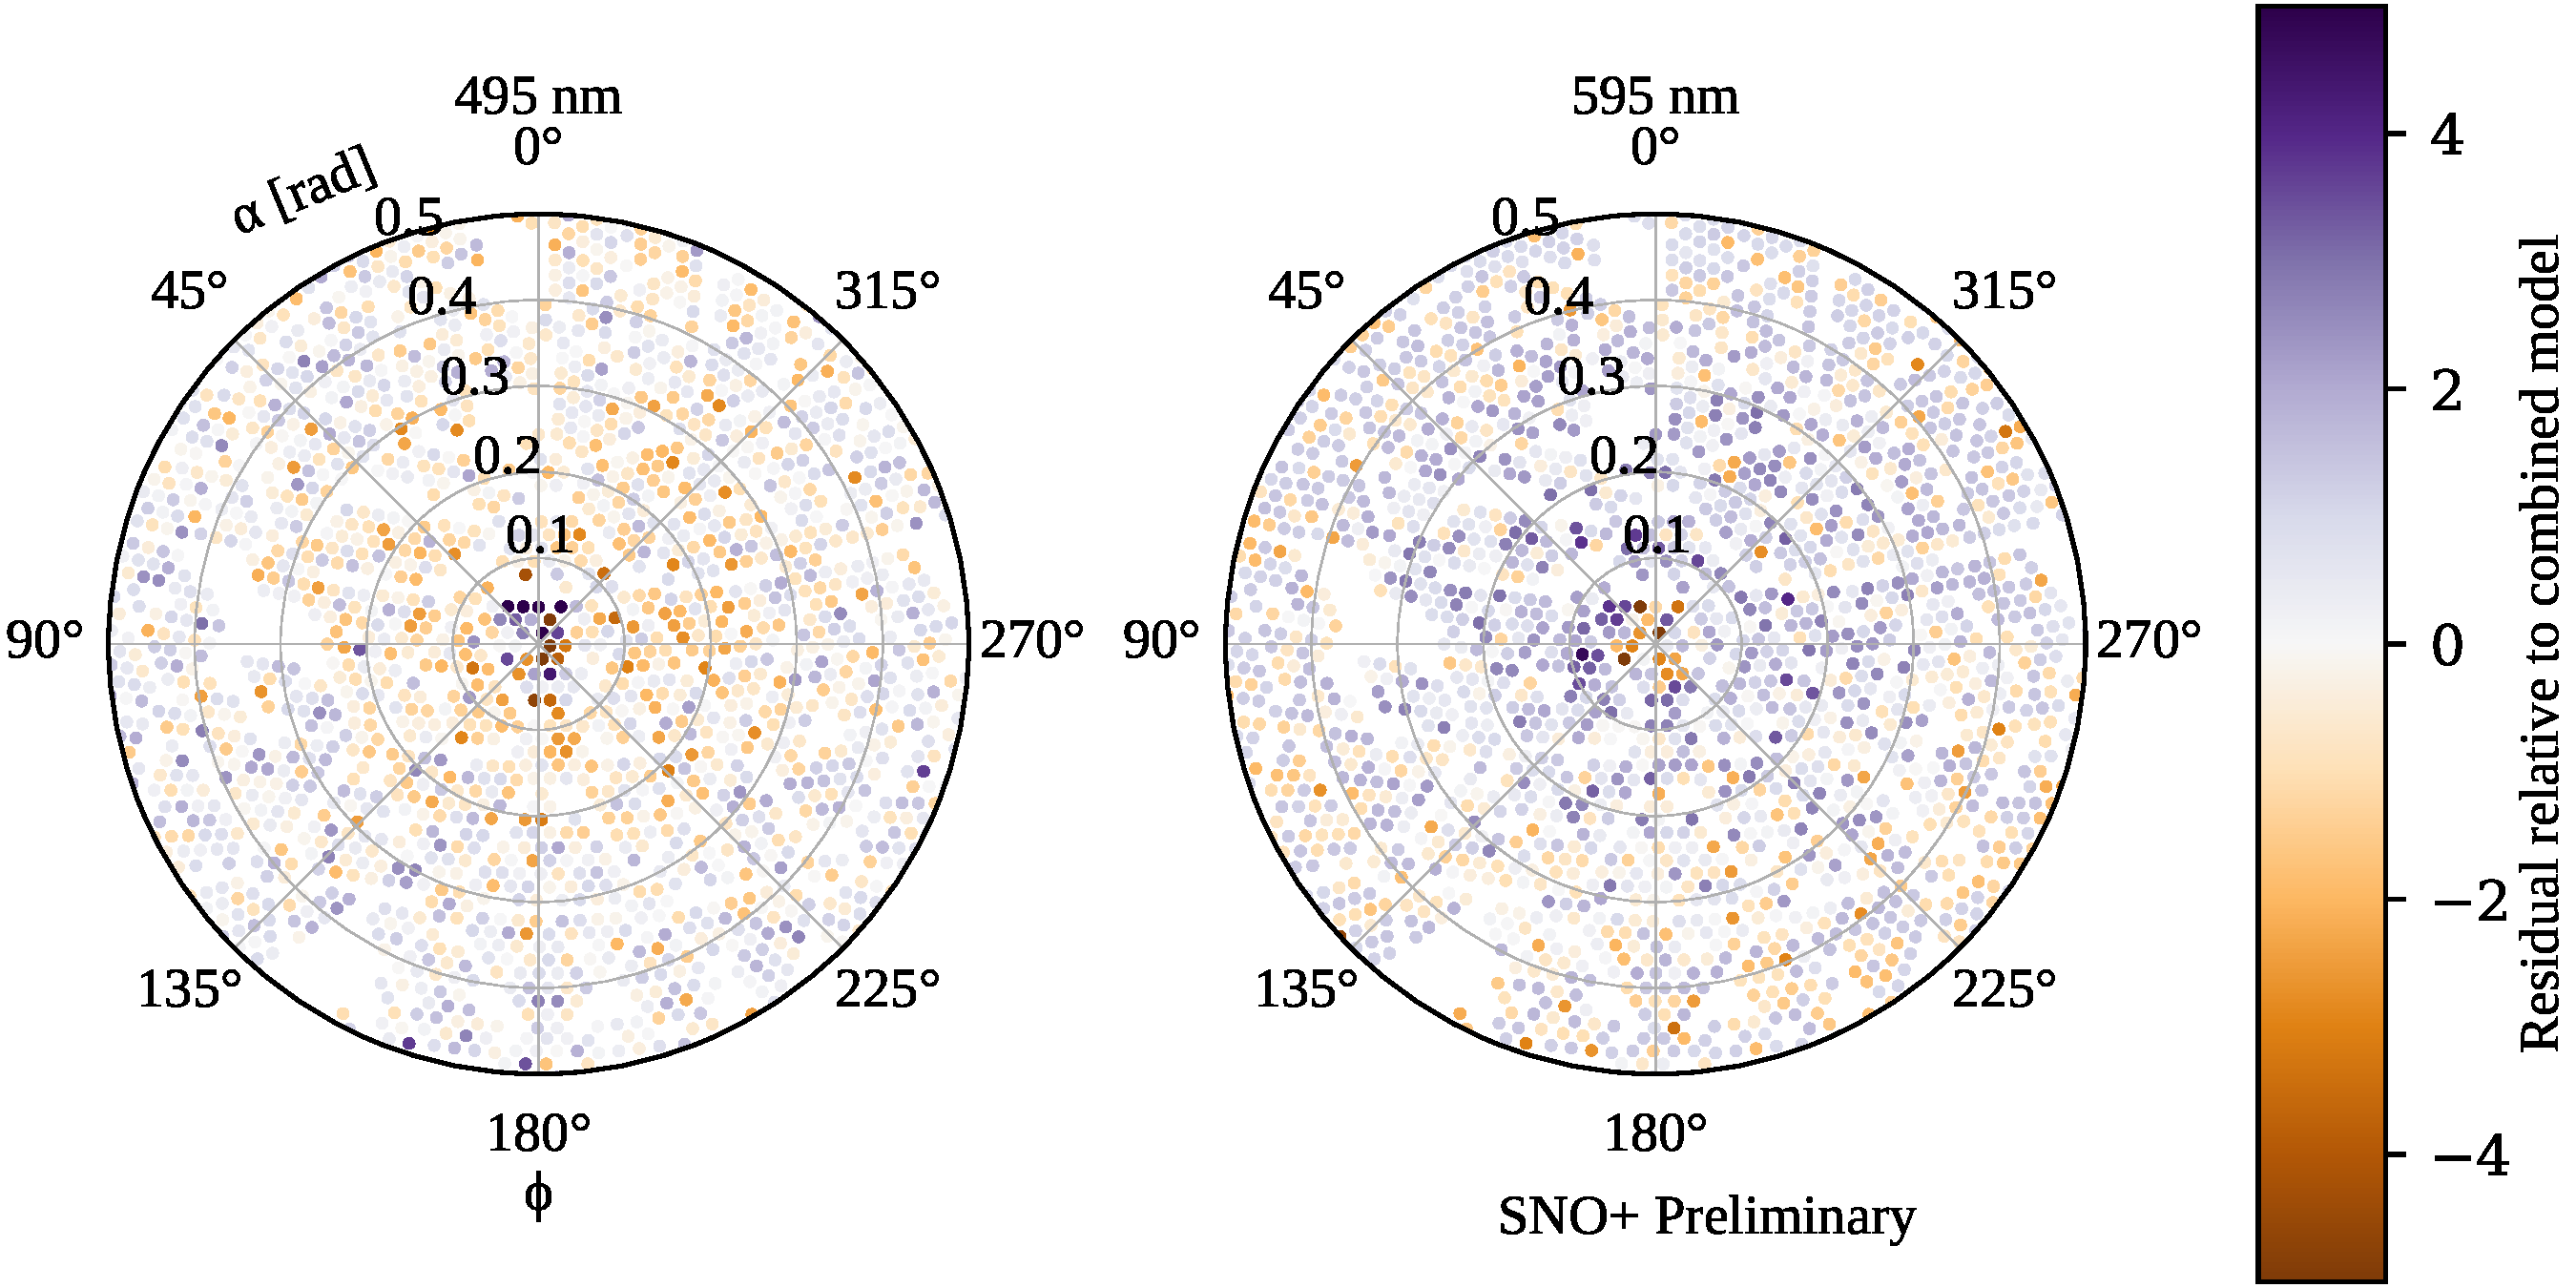
\includegraphics[width=\textwidth]{5_SMELLIESimulation/images/residual_wavelength_comparison_data_model_nice.pdf}
    \caption{Residuals from subruns at two different wavelengths, both compared to the combined beam profile model for fibre FS055. A negative sign, and hence bluer colours, indicate that the combined model underestimates the observed intensity for that particular subrun. Values with a magnitude beyond 5 are shown capped at this maximal value for the purposes of this plot. These PMTs are plotted in the polar fibre coordinates $(\alpha,\phi)$.}
    \label{fig:llr}
\end{figure}
All three of these features --- rope shadows, AV reflections, and wavelength dependence --- add systematic uncertainty to the beam profiles, beyond the statistical uncertainty as measured by the width of the likelihood distribution. Certainly if one wanted to further improve the uncertainties in the beam profiles, tackling these challenges would be key.
% \include{Chapter6/chapter6}
\chapter{Solar Oscillation Analysis}

\section{Analysis Methodology}
     \begin{itemize}
        \item Start with observational principle: changes in oscillation parameters lead to change in the energy spectrum of neutrinos elastically-scattering in the detector, and hence a change in the observed energy spectra of elastically-scattered electrons within the detector. Demonstrate basic impact on modifying $\Delta m^{2}_{21}$ and $\theta_{12}$.
        \item Want to maximise the sensitivity to measuring these two parameters. Energy spectrum of signal is background-free above $\sim\SI{5}{\MeV}$, but rate is substantially larger at lower energies. If one can minimise backgrounds at the lower energies, then there should be hopes of obtaining a measurement with greater precision!
        \item Set up analysis approach: a Bayesian analysis using MCMC. Explain why this was chosen at a high level first: allows for us to perform a relatively complex analysis with multidimensional PDFs, numerous backgrounds, systematics, constraints on parameters, all whilst allowing us to obtain well-defined measures of uncertainty on our final results.
        \item Test statistic: binned extended log-likelihood. Explain why this is fundamentally the ``right''  test statistic to use. Allows for handling of constraints and systematics.
        \item Give an overview of how an MCMC works. Key idea: exploring parameter space in such a way as to reproduce posterior density distribution. Clever! Helps to avoid ``curse of dimensionality'' that often arises in fits with numerous parameters. Must also explain how we work in a fundamentally Bayesian, not frequentist, statistical approach.
        \item Explain background processes we'll be dealing with: can be distinguished by event topology, energy spectrum, and position distribution.
        \item Explain cuts that I am using for the analysis. Demonstrate how these attempt to maximise our signal sensitivity. Leads nicely into choice of 2D fit in both energy and radius (cubed).
        \item Describe implementation of neutrino oscillations within the fitting procedure: flat priors on the oscillation parameters, but a strong constraint from the solar flux. Explain choices of constraint that are possible. MCMC varies oscillation parameters and flux scaling factor, which then modifies the solar signal PDFs through a de-facto systematic that is a function of true neutrino energy, a 3\textsuperscript{rd} ``bookkeeping'' dimension in the signal's PDFs only. Neutrino oscillations simulated via PSelmaa, which accounts for MSW effect in both the Sun and the Earth. For computational speed, at run-time we actually use a lookup table with linear interpolation for the survival probability as a function of parameters.
        \item Implementation of systematics: we handle them generally as linear transformations acting on the vector of bin data. Clever! Which systematics do we expect to be particularly important for this analysis? Well, mismodelling in detector optics etc. can lead to changes in the measured energy spectrum of processes, which can be decomposed into an energy scale term and an energy smearing term to first order. Systematics also possible in the radial dimension (expected to be less important?) 
        
     \end{itemize}

\section{Analysis on Scintillator-Phase data}
\begin{itemize}
    \item Description of dataset chosen for analysis: full-scint data that satisfies the ``gold'' list of run selection requirements, between 1\textsuperscript{st} June 2022 and March 2023. Starting date chosen to ensure radon levels have stabilised within the centre of the detector.
    \item Impact of cuts on data and MC. Show tables (the full details maybe in an appendix) indicating this.
    \item Describe the constraints chosen to apply to the fit, and why they can be justified.
    \item Running \& validation of MCMC fitting. Show plots of parameter values versus step, to demonstrate that the step sizes have been tuned sufficiently. Show auto-correlation plots, to motivate a sensible ``burn-in'' size. Show posterior density plots for each nuisance parameter, to check that they all look sensible and have sufficient statistics. Show plot of correlation coefficients between parameters, and look at any correlations that are particularly interesting.
    \item Look at the data versus MC plot in energy, radius, and both. Is there a good fit to data? Any clear disagreements?
    \item Show 2D contour plot for oscillation parameter posterior density. Note salient features. Show 1D posterior densities for each oscillation parameter. Derive measurement result for $\theta_{12}$.
    \item Show impact of modifying certain constraints on the final results of the measurement of $\theta_{12}$.
\end{itemize}

\section{Sensitivity Projections}


\section{Conclusions}
% \include{Chapter8/chapter8}



% ********************************** Back Matter *******************************
% Backmatter should be commented out, if you are using appendices after References
%\backmatter

% ********************************** Bibliography ******************************
\begin{spacing}{0.9}

% To use the conventional natbib style referencing
% Bibliography style previews: http://nodonn.tipido.net/bibstyle.php
% Reference styles: http://sites.stat.psu.edu/~surajit/present/bib.htm

% \bibliographystyle{apalike}
\bibliographystyle{References/h-physrev5}
%\bibliographystyle{unsrt} % Use for unsorted references  
%\bibliographystyle{plainnat} % use this to have URLs listed in References
\cleardoublepage
\bibliography{References/references} % Path to your References.bib file


% If you would like to use BibLaTeX for your references, pass `custombib' as
% an option in the document class. The location of 'reference.bib' should be
% specified in the preamble.tex file in the custombib section.
% Comment out the lines related to natbib above and uncomment the following line.

% \printbibliography[heading=bibintoc, title={References}]


\end{spacing}

% ********************************** Appendices ********************************

% \begin{appendices} % Using appendices environment for more functunality

% \chapter{Expected Rates and Constraints in the Solar Analysis}\label{chap:appendix_solar_rates}

\section[Boron-8 Signal]{\beight{} Signal}
Numerous theoretical predictions and experimental measurements have been made of the \beight{} flux. For this analysis, two different values have been used. The SSM predicts a relatively loose constraint of $\Phi_{\beight{}} = (5.46\pm 12\%)\times 10^{6}\,\si{\per\cm\squared\per\second}$~\cite{vinyolesB16StandardSolar2018}, % cite SSM flux
whereas a recent global fit of neutrino oscillation experiments by Bergstr\"{o}m \textit{et al} leads to a much stronger constraint of $\Phi_{\beight{}} = (5.16\,^{+2.5\%}_{-1.7\%})\times 10^{6}\,\si{\per\cm\squared\per\second}$~\cite{bergstromUpdatedDeterminationSolar2016}. % cite Bergstrom et al
We shall mainly use the latter result to both calculate the expected rate of the signal events in the detector, and the fractional uncertainties used to constrain this rate. The looser constraint coming from the SSM will be used for comparison.

To calculate the number of electrons within the liquid scintillator, the method used in~\cite{inacioDataAnalysisWater2022} is followed, % cite Ana Sofia's thesis
which uses the formula:
\begin{equation}
    n_{e} = \frac{\left(f_{\mathrm{LAB}}n_{\mathrm{LAB}} +
                        f_{\mathrm{PPO}}n_{\mathrm{PPO}}\right)
                  N_{A}M_{\mathrm{LAB}}}
                 {m}.
\end{equation}
Here, $f_{\mathrm{LAB}}$ and $f_{\mathrm{PPO}}$ are the fraction by weight of the LAB and PPO within the scintillator cocktail, respectively. Because this analysis uses data taken during the scintillator phase with a PPO concentration of \SI{2.2}{\g} for every litre of LAB, these take values 99.744\% and 0.256\%, respectively. $n_{\mathrm{LAB}}$ and $n_{\mathrm{PPO}}$ are the mean number of electrons per molecule of LAB and PPO, respectively. PPO has the chemical formula \ce{C_{15}H_{11}NO}, leading to $n_{\mathrm{PPO}} = 116$. The LAB used in SNO+ has varying alkyl chain lengths, leading to a varying number of electrons per molecule. This distribution is known to have changed between batches of LAB made by the manufacturer, and is also impacted by the distillation process used during the purification of the LAB before it was put into the AV. At the time of writing, no final molecular breakdown has been made for the LAB within the detector; for now the breakdown provided here has been used~\cite{lebeufLABCertificateAnalysis2020}, % cite LAB breakdown DocDB #7572
from a representative tanker truck of LAB: there $n_{\mathrm{LAB}} = 131.68$. Finally, $N_{A} = \SI{6.02e23}{\per\mol}$ is Avogadro's Constant, $M_{\mathrm{LAB}} = \SI{780.2}{\tonne}$ is the total mass of scintillator within a sphere of radius the size of the AV, and $m = \SI{235}{\g\per\mol}$ is the molecular weight of the scintillator. This leads to a value for the number of electron targets:
\begin{equation*}
    n_{e} = \num{2.63e32}\; \mathrm{electrons}.
\end{equation*}

Eq.~\ref{eq:solar_rate} can be modified to get an equation for the total rate of solar neutrino events by flavour, before oscillations or analysis cuts are considered:\
\begin{equation}
    R_{i} = \Phi_{\beight{}}n_{e}
                \int S_{\nu}\left(E_{\nu}\right)\sigma_{\nu_{i}}\left(E_{\nu}\right)\,dE_{\nu}.
\end{equation}

Using the cross-section formula from Eq.~\ref{eq:enu_es_xsec}, the \beight{} spectral shape from~\cite{winterB8NeutrinoSpectrum2006}, and $\Phi_{\beight{}} = \SI{5.46e6}{\per\cm\squared\per\second} \left(\SI{5.16e6}{\per\cm\squared\per\second}\right)$, the expected rate before considering oscillations or cuts is:
\begin{equation*}
    R_{i} = 
    \begin{cases}
        2743.2 (2592.5)\; \text{events/yr} & \quad \text{for } i = e,\\
        489.7 (462.8)\;  \text{events/yr} & \quad \text{for } i = \mu,\tau.
    \end{cases}
\end{equation*}
In the above rates, an additional volume correction factor of 1.0139 has been included, because in MC events are simulated within the neck of the AV in addition to the main spherical bulk~\cite{caravacaValidationSNOProduction2019}. % cite Javi, DocDB 5519

\section[Internal Uranium- and Thorium-Chain Backgrounds]{Internal Uranium- and Thorium-Chain\\Backgrounds}
As mentioned in Section~\ref{sec:u_th_internals}, \ce{^{214}Bi-Po} and \ce{^{212}Bi-Po} decays, coming from the \ce{^{238}U} and \ce{^{232}Th} decay chains respectively, are capable of generating distinctive delayed coincidence events. Rafael Hunt-Stokes was able to use a series of cuts to isolate both types of coincidence signals~\cite{hunt-stokesUraniumThoriumBackground2022}, % cite Rafa's tech note?
looking at coincidence signals within the same \SI{5.0}{\m} FV as this analysis. After correcting for his cut efficiencies, he obtained a derived rate in the whole detector of~\cite{hunt-stokesPrivateCommunication2023}: % cite Rafa
\begin{equation*}
    \text{BiPo rate} = 
    \begin{cases}
        0.94\; \text{events/hour} & \quad \text{for } ^{212}\text{Bi-Po},\\
        6.06\; \text{events/hour} & \quad \text{for } ^{214}\text{Bi-Po}.
    \end{cases}
\end{equation*}
These rates assume a uniform concentration of \ce{^{222}Rn} and \ce{^{220}Rn} throughout the detector: this is how internal backgrounds are simulated by default in \texttt{RAT}. However, it has been shown that this is not at all the case within SNO+; radon ingress from the AV neck propagates through the bulk of the detector via convection currents induced by the thermal gradient present throughout the detector~\cite{wilsonThermallydrivenScintillatorFlow2023}. % Cite John wilson's paper, JoshW's & Rafa's tagging
This radon ingress also breaks the secular equilibrium of the two decay chains, so that one can no longer make straightforward predictions about rates for decays in the chains above radon. Fortunately for this analysis, Table~\ref{tab:MC_cut_effs} showed that the cut efficiencies for \ce{^{228}Ac} and \ce{^{234m}Pa} decays, both in their respective decay chain above radon, are negligible. This means that even if their decay rates were much greater than what would be predicted from the tagged BiPo rates, a negligible number of events are expected for both in the livetime of the dataset considered in this analysis.

The combination of broad coincidence tagging as well as using an in-window BiPo classifier cut ensures that the expected rate of \ce{Bi-Po} events that survive all the cuts is 1.5 and 2.5 for \ce{^{212}Bi-Po} and \ce{^{214}Bi-Po}, respectively. Because the branching ratio of \ce{^{212}Bi\to^{208}Tl} is 36\%, and the branching ratio of \ce{^{214}Bi\to^{210}Tl} is 0.021\%~\cite{martinNuclearDataSheets2007,shamsuzzohabasuniaNuclearDataSheets2014}, % cite some table of decays
after considering the cut efficiencies in this analysis 512.4 internal \ce{^{208}Tl} and 1.1 internal \ce{^{210}Tl} events are expected.

In theory, the non-uniformity of all the radon-induced backgrounds could impact the results of the oscillation analysis. However, the small rates of each of these backgrounds after cuts have been applied indicated that only the internal \ce{^{208}Tl} could plausibly have any effect. For this particular background, each slice of the binned PDF in $r_{3}$ was allowed to float independently, with no constraints. The other three related backgrounds considered in the fit (\ce{^{210}Tl}, \ce{^{212}Bi-Po}, and \ce{^{214}Bi-Po}) did not have this PDF splitting applied to them. A loose 25\% constraint on each of these three processes' rates was applied, to account for the current uncertainty in the calculation of R. Hunt-Stokes' tagging efficiency.

\section[Alpha-n Reactions]{\alphan{} Reactions}
As discussed in Section~\ref{sec:alphans}, \alphan{} reactions are induced by $\alpha$-particles generated in the detector. In the SNO+ scintillator phase, the dominant source of $\alpha$-particles are decays of \ce{^{210}Po} located both within the scintillator and on the AV surfaces. Because of substantial quenching by the scintillator, the reconstructed energy of the \ce{^{210}Po} $\alpha$ events fall substantially below $E_{\textrm{min}}$. The rate of the internal and surface \ce{^{210}Po} events have been tracked throughout the scintillator phase by Serena Riccetto and Shengzhao Yu, respectively.

Within the \SI{5}{\m} FV, S. Riccetto measured a total of \num{1.60e8} \ce{^{210}Po} events over the runs considered for this analysis~\cite{riccettoPrivateCommunication2023,riccettoFullFillInternal2023}. % cite Serena (private comm?)
Assuming the internal rate of these events are uniform throughout the scintillator, this leads to a total rate of \num{2.78e8} events for all the scintillator. After using a conversion rate of \num{6e-8} neutrons generated per $\alpha$ on \ce{^{13}C} in liquid scintillator~\cite{morton-blakeFirstMeasurementReactor2021,lozzaNeutronSourcesBackgrounds2015}, % where did this come from?
the expected number of internal \alphan{} events before cuts is 17. However, because a coincidence cut is used in this analysis, the vast majority of these should be removed, leading to merely 0.009 events expected after cuts.

Similarly, S. Yu measured the surface \ce{^{210}Po} rate to vary between \SIrange{2}{5}{\Bq\per\square\metre} over the time period of this analysis as well as a function of height in the detector~\cite{yuAVSurfacePo2102023}. % cite Shengzhao's work
Using the midpoint value of \SI{3.5}{\Bq\per\square\metre}, one can derive an expected rate of 554.4 surface \alphan{} events occurring over the dataset's livetime, before cuts. Once again, the coincidence cut as well as the FV cut removes the vast majority of these events, so that only 0.07 events are expected after all cuts have been applied. Because both classes of \alphan{} events have negligible expected rates in the dataset, they were not included within the MCMC fit.

\section{External Backgrounds}\label{sec:rates_ext_backgrounds}
During the water phase of SNO+, an analysis of the rates of the external backgrounds was performed by Tony Zummo~\cite{zummoExternalBackgroundBox2022}. % cite Zummo's externals results
The results of this analysis are shown in Table~\ref{tab:externals_rates_zummo}, giving the measured rates as a fraction of the nominal values given in~\cite{andringaCurrentStatusFuture2016}. % cite white paper.
Although the statistical uncertainty for these measurements were quite small, the total systematic uncertainty was substantial because T. Zummo's analysis involved looking at events in the tail of energy distributions, so that any uncertainty in the energy scale systematic had a strong impact on the number of events observed within the tail. These measured rates and their systematic uncertainties were used to predict the expected rate and constrain the external backgrounds in this scintillator phase solar analysis. For the AV, ropes, and PMTs, this seems reasonable as we do not expect there to be any substantial change in these backgrounds between the phases. The exception to this is the external water, where various aspects of the water purification process have changed over the years since T. Zummo's analysis dataset was taken~\cite{kaptanogluFirstLookExternal2023}. Because of this, the water phase measured rate was used as a starting point for the fit, but no constraint was applied.

\begin{table}
    \centering
    \begin{tabular}{c r}
        \hline
        Background Type & Rate (Fraction of Nominal)  \\ \hline \hline
        AV \& Ropes    & $0.21\pm0.009^{+0.64}_{-0.21}$  \\
        External Water & $0.44\pm0.003^{+0.32}_{-0.27}$  \\
        PMTs           & $1.48\pm0.002^{+1.65}_{-0.60}$  \\
        \hline
    \end{tabular}
    \caption[Measured rates of the external backgrounds during the water phase of SNO+, by Tony Zummo]
    {Measured rates of the external backgrounds during the water phase of SNO+, by Tony Zummo~\cite{zummoExternalBackgroundBox2022}. % cite Zummo
    }
    \label{tab:externals_rates_zummo}
\end{table}

Before the expected number of triggered events can be calculated for each external background process, two subtleties must be dealt with. Firstly, MC production of the externals did not include the hold-up ropes at the time of performing the analysis. This is not a major problem, because the hold-up ropes are of substantially lower mass than the hold-down ropes, and also their average radius from the centre of the detector is much larger. This means that the expected rate of events from the hold-up ropes that manage to reconstruct inside the FV should be sub-dominant to their hold-down counterparts. For the purposes of this thesis, the combined rate for both kinds of ropes were calculated assuming the same rate of decays per unit volume, with the overall cut efficiency and derived PDFs coming from just the hold-down ropes.

Secondly, because the attenuation length of a \SI{2.6}{\MeV} $\gamma$ particle is \SI{23}{\cm} in water~\cite{bergerXCOMPhotonCross2009,heintzelmanSurvivalRadiiPSUP2012}, % cite xsec database (see W.Heintzelman DocDBs!)
the vast majority of external backgrounds which start from a substantial distance away from the AV do not generate $\gamma$s that make it into the scintillator. As a result, an enormous amount of computational resources could be wasted on simulating events that never get into the ROI. To work around this, PMT $\beta-\gamma$ events are modelled as \SI{2.6}{\MeV} $\gamma$s generated at a radius of \SI{6.2}{\m} (just outside the AV), pointing radially inwards. Making some basic assumptions about these events, one can derive the expected survival rate of these $\gamma$ particles as a function of radius~\cite{heintzelmanSurvivalRadiiPSUP2012,heintzelmanAngularDistributionSurviving2013}. % cite Heintzelman #1712, 1729
This leads to a correction factor of \num{1.17e-6} being applied to the results of the radial shell simulation.

Similarly, simulations of background events in the external water and ropes are restricted from starting beyond certain maximum radii. The particular maximum radius chosen depends on the specific process, in order to ensure a negligible impact on the fraction of simulated events that actually deposit any energy into the scintillator. This leads to rate correction factors of 0.35 and 0.50 for external water \ce{^{214}Bi} and \ce{^{208}Tl} events, as well as 0.50 and 0.35 for hold-down and hold-up ropes~\cite{inacioUsingSmallerShell2019}. % cite Ana Sofia's DocDB #5154
% \include{Appendix2/appendix2}

% \end{appendices}

% *************************************** Index ********************************
% \printthesisindex % If index is present

\end{document}
